Referred to \cite{CMS-PAS-HIG-19-001}.
%
%Vector Boson Fusion (VBF) and other production mechanisms of Higgs Boson normally differ as regards the jet kinematics. 
%In this analysis, jets are thus used for the event categorization, which will be introduced in Section~\ref{sec:categorization}.
%
%\subsubsection{Jet Identification}
%
%Jets are reconstructed by using the anti-$k_T$ clustering algorithm out of particle flow candidates, with a distance parameter $R = 0.4$, 
%after rejecting the charged hadrons that are associated to a pileup primary  vertex.
%
%To reduce instrumental background, the tight working point jet ID suggested by the JetMET Physics Object Group is applied~\cite{JetID2018}. 
%In addition, jets from Pile-Up are rejected using the PileUp jet ID criteria suggested by the JetMET POG~\cite{JetPUID2017}.
%It is to be noted that the PU JetID was only derived for 2016 conditions but is also applied to 2017 and 2018 samples. 
% 
%In this analysis, the jets are required to be within $|\eta| < 4.7$ area and have a transverse momentum above 30 GeV. 
%In addition, the jets are cleaned from any of the tight leptons (passing the SIP and isolation cut computed after FSR correction) 
%and FSR photons by a separation criterion: $\Delta R(\text{jet,lepton/photon}) > 0.4$.
%
%\subsubsection{Jet Energy Corrections}
%
%The calorimeter response to particles is not linear
%and it is not straightforward to translate the measured jet energy
%to the true particle or parton energy, therefore we need Jet Energy Corrections.
%In this analysis, standard jet energy corrections are applied to the reconstructed jets,
%which consist of L1 Pileup, L2 Relative Jet Correction,
%L3 Absolute Jet Correction for both Monte Carlo samples and data,
%and also residual calibration for data~\cite{JECMC2018}.
%
%The table~\ref{tab:jecjer} summarizes the various JEC and JER tags used in this analysis.
%
%\begin{table}[h!]
%%\scriptsize
%    \centering
%    \begin{tabular}{c|c c }
%%\hline
%%\multicolumn{4}{|c|}{2016 Datasets} 
%%\multicolumn{4}{|c|}{2016 Datasets}
%       & JEC tag & JER tag      \\
%\hline %----------------------------------------------------------------------------------------
%2016 & Summer16\_07Aug2017All\_V11 & Summer16\_25nsV1\_MC \\
%\hline %----------------------------------------------------------------------------------------
%2017 & Fall17\_17Nov2017\_V32\_94X & Fall17\_V3\_94X\_MC \\
%\hline %----------------------------------------------------------------------------------------
%2018 & Autumn18\_RunABCD\_V19 & Autumn18\_V7\_MC \\
%\hline %----------------------------------------------------------------------------------------
%
%%minimum BDT score    &  $|\eta| < 0.8 $ & $0.8 < |\eta| < 1.479$ 	& $|\eta| > 1.479$      \\
%%\hline %----------------------------------------------------------------------------------------
%%$ 5 < p_T < 10 $ GeV &  0.9503      & 0.9461  	& 0.9387		\\
%%$p_T > 10$ GeV         &  0.3782	& 0.3587		&  -0.5745	\\
%%\hline %----------------------------------------------------------------------------------------
%%\hline %----------------------------------------------------------------------------------------
%     \end{tabular}
%\small
%    \caption{Summary of all JEC and JER tags.}% \textbf{FIXME: WP to be defined!}}
%    \label{tab:jecjer}
%\end{table}
%
%% PUT the versions of the JEC/JER
%
%
%% \textbf{At the moment only preliminary version of JEC for MC is available. As recommended no JEC is applied to data.}
%%Jet Energy Resolutions corrections are, however, NOT applied to 2018 samples (see discussion below).
%
%\subsubsection{Additional criteria on jets}
%\label{sec:jetstudies}
%The three data taking periods analyzed in this note suffered from issues during the data taking which impact the quality of the jet reconstruction. Some of these issues would need a complete re-reconstruction of the data to be fully fixed (the so-called ``Ultra Legacy ReReco''), which is beyond the scope of the paper. In the mean time, following the guidance from the JetMET POG, we studied the possibilty of adding some criteria on the jet to cope with these issues. 
%
%\paragraph{L1 pre-firing}
%
%In 2016 and 2017, the gradual timing shift of ECAL was not properly propagated to L1 trigger primitives (TP) resulting in a significant fraction of high eta TP being mistakenly associated to the previous bunch crossing. Since Level 1 rules forbid two consecutive bunch crossings to fire, an unpleasant consequence of this (in addition to not finding the TP in the bx 0) is that events can self veto if a significant amount of ECAL energy is found in the region of $2<|\eta|<3$. This effect is not described by the simulations~\cite{L1PrefiringTwiki}. A weight is thus calculating for each event, not to prefire, and apply to the simulation in 2016 and 2017 samples. The official tool is used for this purpose~\cite{L1PrefiringTwiki}.
%
%The Fig~\ref{fig:jetL1} shows the impact of the L1 pre-firing weights on the signal MC. As expected, the effect on ggH samples is minor but is at the leve of 2-3\% in the endcaps for VBF production mode. 
%
%\paragraph{removal of noisy jets}
%
%Increased jet multiplicity was reported for 2017 data, creating ``horns'' in the jet $\eta$ distribution for $2.5<\eta_{jet}<3$ (FIXME: add ref). The issue was linked to an increase of the ECAL noise, PU and bunch-crossing dependant, thus getting worse as luminosity increases. The problem can only be fixed in the UL ReReco. For now, we checked the impact of rejecting jets with raw $p_T<50$ GeV in 2.65 $< \eta <$ 3.139. As we see no significant impact in the data/MC agreement, we decided not to use these cuts.
%
%\paragraph{HEM 15/16 failures}
%
%Following	a CMS-wide power interlock, the power-on of CAEN A3100HBP modules that provide low-voltage power to the on-detector HE front-end electronics led to irreversible damage of two sectors on the HE minus side, HEM15 and HEM16 (FIXME: add ref). No significant impact was seen and nothing particular is done to cope with this. 
%
%%https://twiki.cern.ch/twiki/bin/view/CMS/HIGJetMET#Known_JetMET_issues 
%
%\begin{figure}[!h]
%\centering
%
%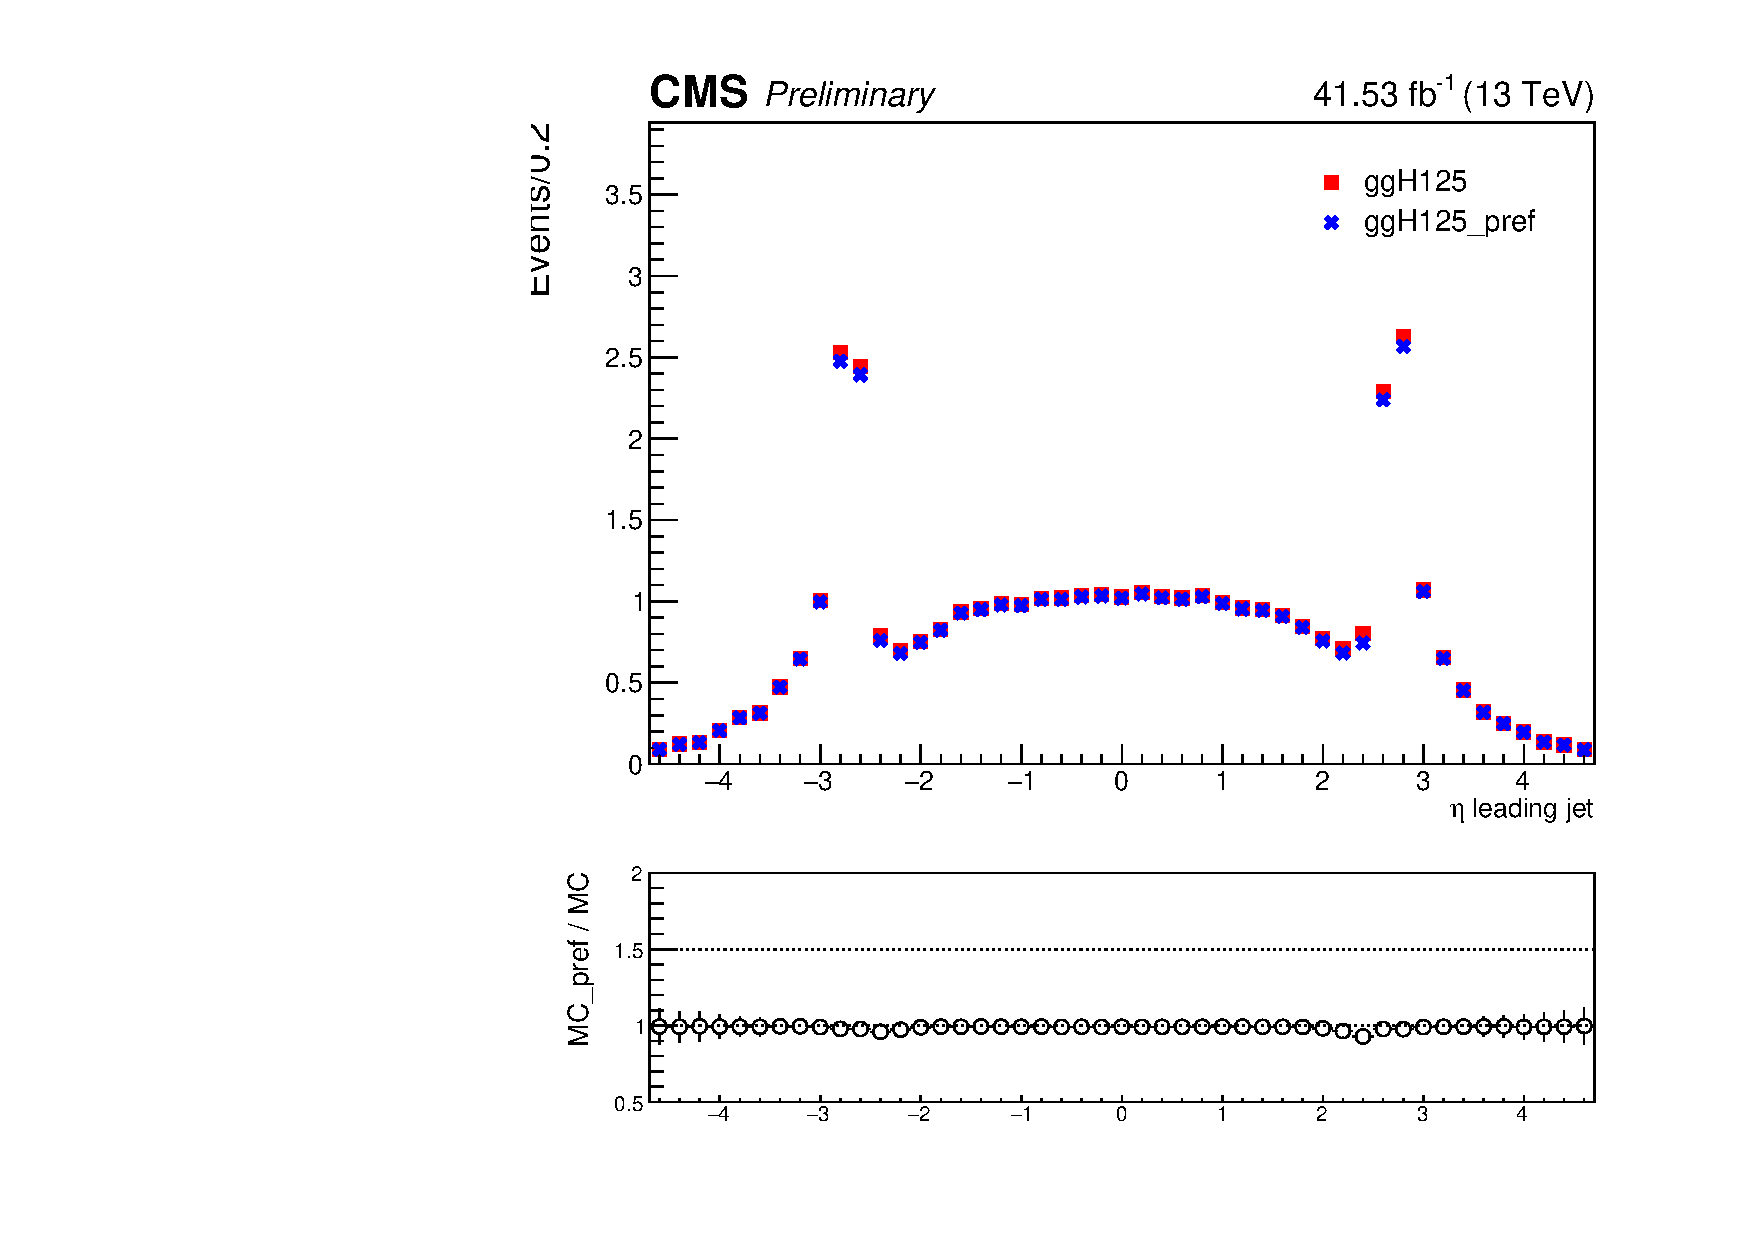
\includegraphics[width=0.49\linewidth]{Figures/Jets/JetEta_GGH_data2017_ZZTree_ratio.pdf} 
%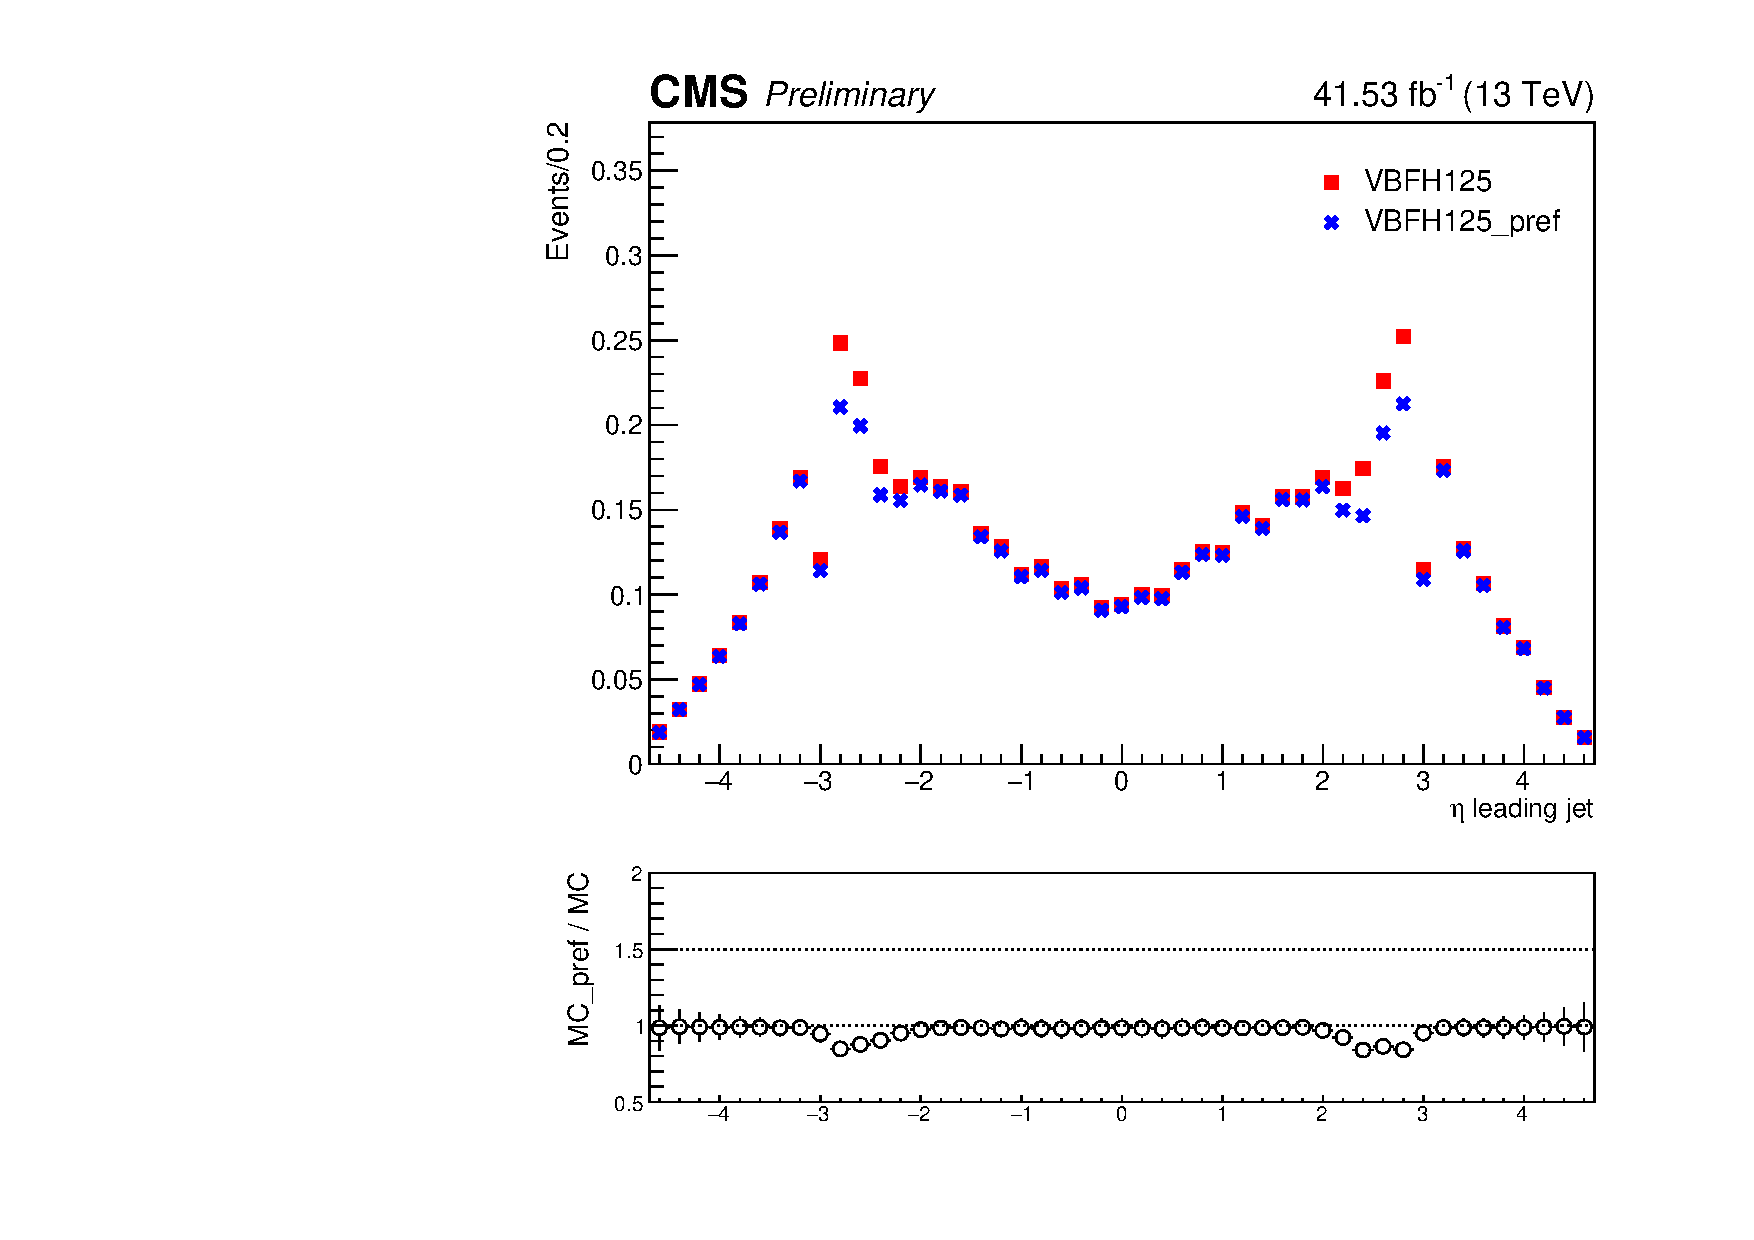
\includegraphics[width=0.49\linewidth]{Figures/Jets/JetEta_VBF_data2017_ZZTree_ratio.pdf} \\
%\caption{Comparison between 2017 MC samples with (blue) and without (red) L1 pre-firing weights for ggH (left) and VBFH signals. The ratio is shown at the bottom of each plot.
%%   (data and MC for number of jets with $p_T>30$~GeV (top) and leading jet $\eta$ (bottom) in Z$\rightarrow \ell\ell$ +jets events.
%% (left) and Z$\rightarrow\mu\mu$ + jets events (right). 
%%MC is normalized to data. Jet ID and Jet PUID are applied. MC samples include DY and ttbar. Data/MC ratio plots are shown in the bottom of each plots, together with the uncertainties (shaded histograms) from Jet Energy Corrections.
%%\textbf{FIXME: Add the uncertainty band in the ratio plot.}
%\label{fig:jetL1}}
%\end{figure}
%
%\subsubsection{B-tagging}
%
%For categorization purpose, we need to distinguish whether a jet is b-jet or not.
%The \emph{DeepCSV} algorithm is used as our b-tagging algorithm. It combines the same information as the previous tagger \emph{CSVv2}, impact parameter significance, secondary vertex and jet kinematics but uses information of more tracks. Also, the b-tag output discriminator is computed with a Deep Neural Network. 
%In this analysis, a jet is considered to be b-tagged if it passes the \emph{medium} working point, i.e. if its $|$ pfDeepCSVJetTags:probb + pfDeepCSVJetTags:probbb $|$ discriminator is greater than 0.4184~\cite{BTAG2018}.
%
%Data to simulation scale factors for b-tagging efficiency are provided for this working point for the full dataset as a function of jet $\pt$, $\eta$ and flavour.
%They are applied to simulated jets by downgrading (upgrading) the b-tagging status of a fraction of the b-tagged (untagged) jets that have a scale factor smaller (larger) than one. %\textbf{They are not yet available but will be applied as soon as they arrive.}
%
%\subsubsection{Missing Transverse Energy}
%MET is not used in this analysis to, for instance, categorize events.
%
%\subsubsection{Validation on data}
%Similarly to what was done with electrons and muons, we performed some validation studies to probe the agreement between data and simulated samples for jets. 
%Events containing $\Zee$ or $\cPZ\rightarrow\cP\mu^{+}\cP\mu^{-}$ were selecting, following the same trigger and lepton selection criteria of the main analysis, but increasing the $p_T$ threshold on leptons  to 30~GeV and asking the invariant mass of the two leptons to be within the 70-110~GeV range.
%
%Basic properties of additional jets in the event,  with $p_T>30$~GeV and $\eta<4.7$, were then compared. Figure~\ref{fig:jets} shows the pseudo-rapidity and transverse momentum of the leading jet in data and MC for the three data taking periods. Fig~\ref{fig:jetsN} shows the jet multiplicity.
%%For 2018, the plots are shown with and without the application of the Jet Energy Resolution corrections. As the current JER seems to promote too much low momenta jets in the endcaps, creating huge horns, we decided not to use JER in 2018 (but we keep the associated uncertainty). 
%%the number of jets and the pseudo-rapidity of the leading jet in data and MC. Simulated samples of Drell-Yan and $\ensuremath{\cPqt\bar{\cPqt}}$ are used. 
%Uncertainties from the jet energy corrections are also displayed on the data/MC ratio plots. % (FIXME: Currently, only 2017 uncertainties are available). 
%
%The agreement between data and simulation is found to be good for the jet transverse momentum or pseudo-rapidity, given the large uncertainties in the forward region. 
%%Jet Energy Scale corrections are applied to both DATA and MC, following the recommendation from JetMET POG but not Jet Energy Resolution corrections. Residual Corrections to DATA have just been released and are therefore not yet included in these plots. We do expect it will improve the data/MC agreement together with increased systematic uncertainties to cover the disagreement in the forward region.
%%Given that no Jet Energy Scale corrections for DATA were available at the time when the plots were made, it is hard to draw definite conclusion on the data/MC agreement. 
%%Simulation is well reproducing the data, apart from the very forward region ($\eta>4$) but the observed discrepancy is well within the uncertainties.
%
%%The leading jet $p_T$ and PFMET distribution are shown in Fig~\ref{fig:met}. The disagreement between data and MC for the MET distribution prevents us at this stage to use this variable in the analysis, in particular to better target VH events where, for instance, a Z would decay into neutrinos.
%%It shows a clear shift between data and MC. The problem is currently under investigation with MET experts. The disagreement is more pronounced in the last data taking period (Run F). The current studies are pointing to an excess of low $p_T$ neutral particles (photon and hadrons) in the endcap, likely due to a combination of time-dependant ECAL transparency loss and underestimation of Out-of-Time PU subtraction (see~\cite{METfix}).
%%REF: https://indico.cern.ch/event/722467/contributions/2971253/attachments/1635662/2609542/MetStudyInZ_18Apr2018_SamuelMay.pdf
%%A first fix was proposed: recompute MET excluding neutrals within $2.5 < \eta < 3$. The corresponding recalculated MET is shown in Fig~\ref{fig:met}. Altough one can see an improvement with respect to the original distribution, the level of agreement between data and MC, especially above 100 GeV, prevents us to use this observable. We thus decided to drop for now the category called ``VH-MET'', targeting the production of Higgs in association with a vector boson with large MET ($>100 $~GeV was required). 
%% as well as the missing transvere energy (MET) in data and MC.  On the other hand, the MET distribution shows a clear shift between data and MC. This is currently under investigation with MET experts.
%%We thus don't expect a perfect agreement with data for high jet multiplicity, high MET value or high b-tag score. 
%
%\begin{figure}[!h]
%\centering
%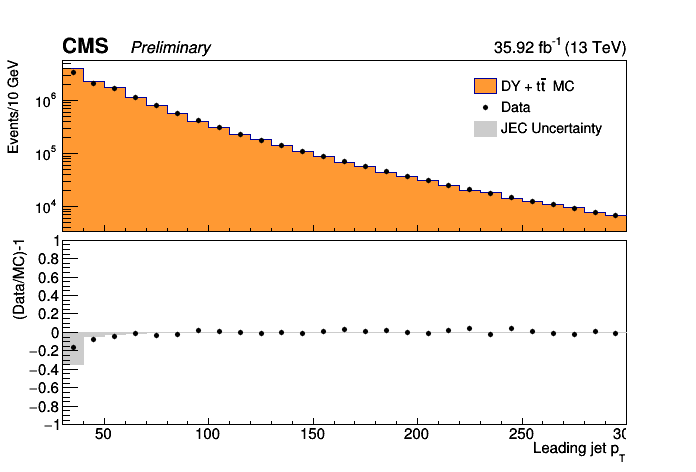
\includegraphics[width=0.49\linewidth]{Figures/Jets/leadingJet_Pt_2016June24.png}
%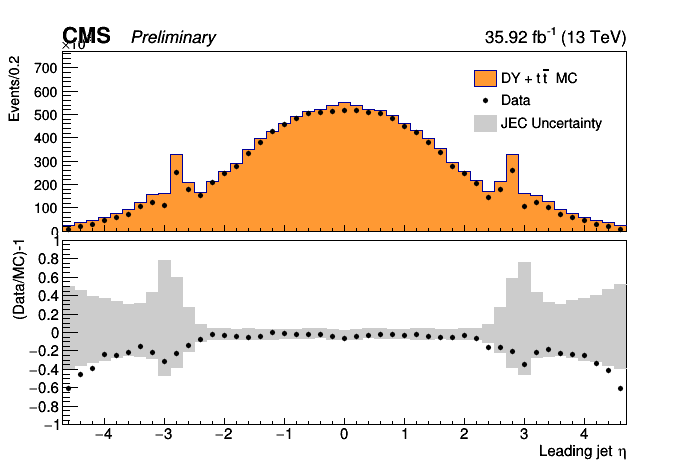
\includegraphics[width=0.49\linewidth]{Figures/Jets/leadingJet_Eta_2016June24.png} \\
%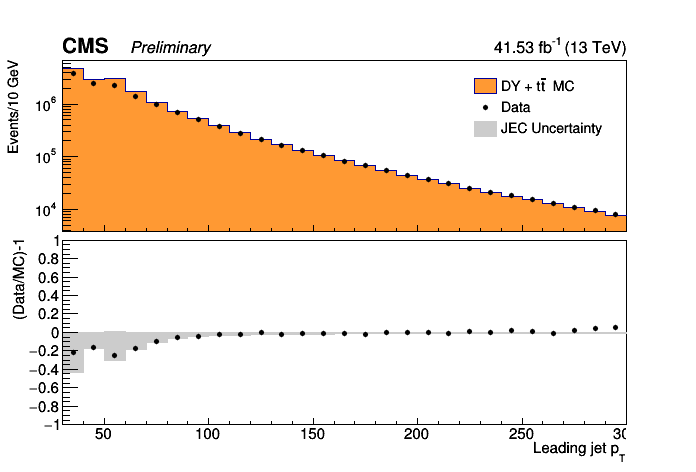
\includegraphics[width=0.49\linewidth]{Figures/Jets/leadingJet_Pt_2017June24.png}
%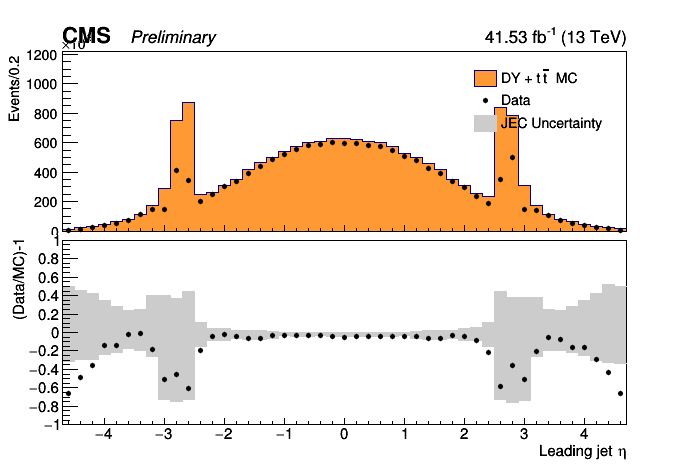
\includegraphics[width=0.49\linewidth]{Figures/Jets/leadingJet_Eta_2017June24.png} \\
%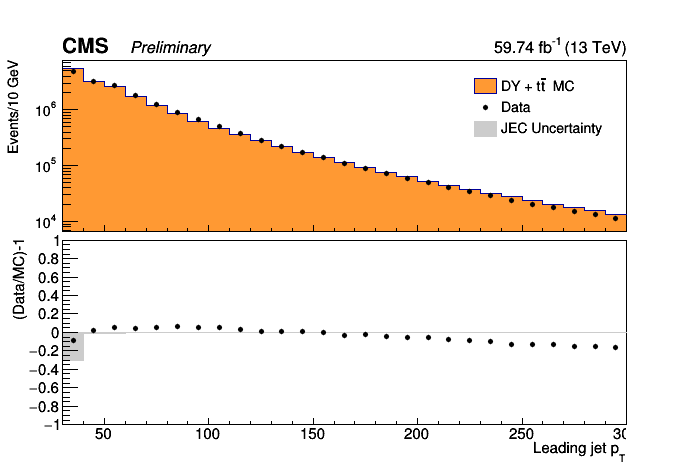
\includegraphics[width=0.49\linewidth]{Figures/Jets/leadingJet_Pt_2018June24.png}
%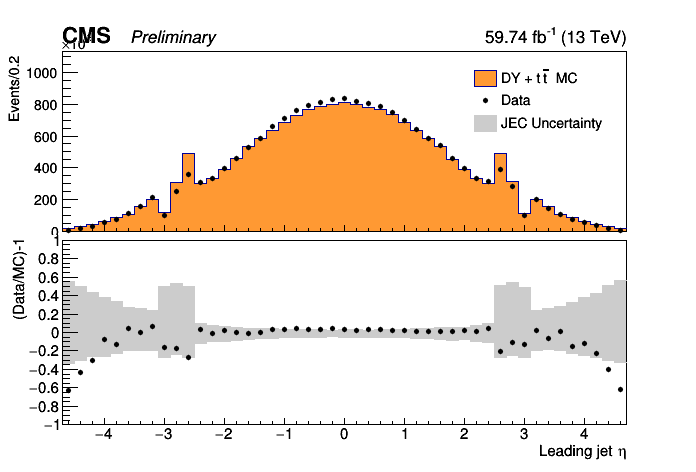
\includegraphics[width=0.49\linewidth]{Figures/Jets/leadingJet_Eta_2018June24.png} \\
%
%%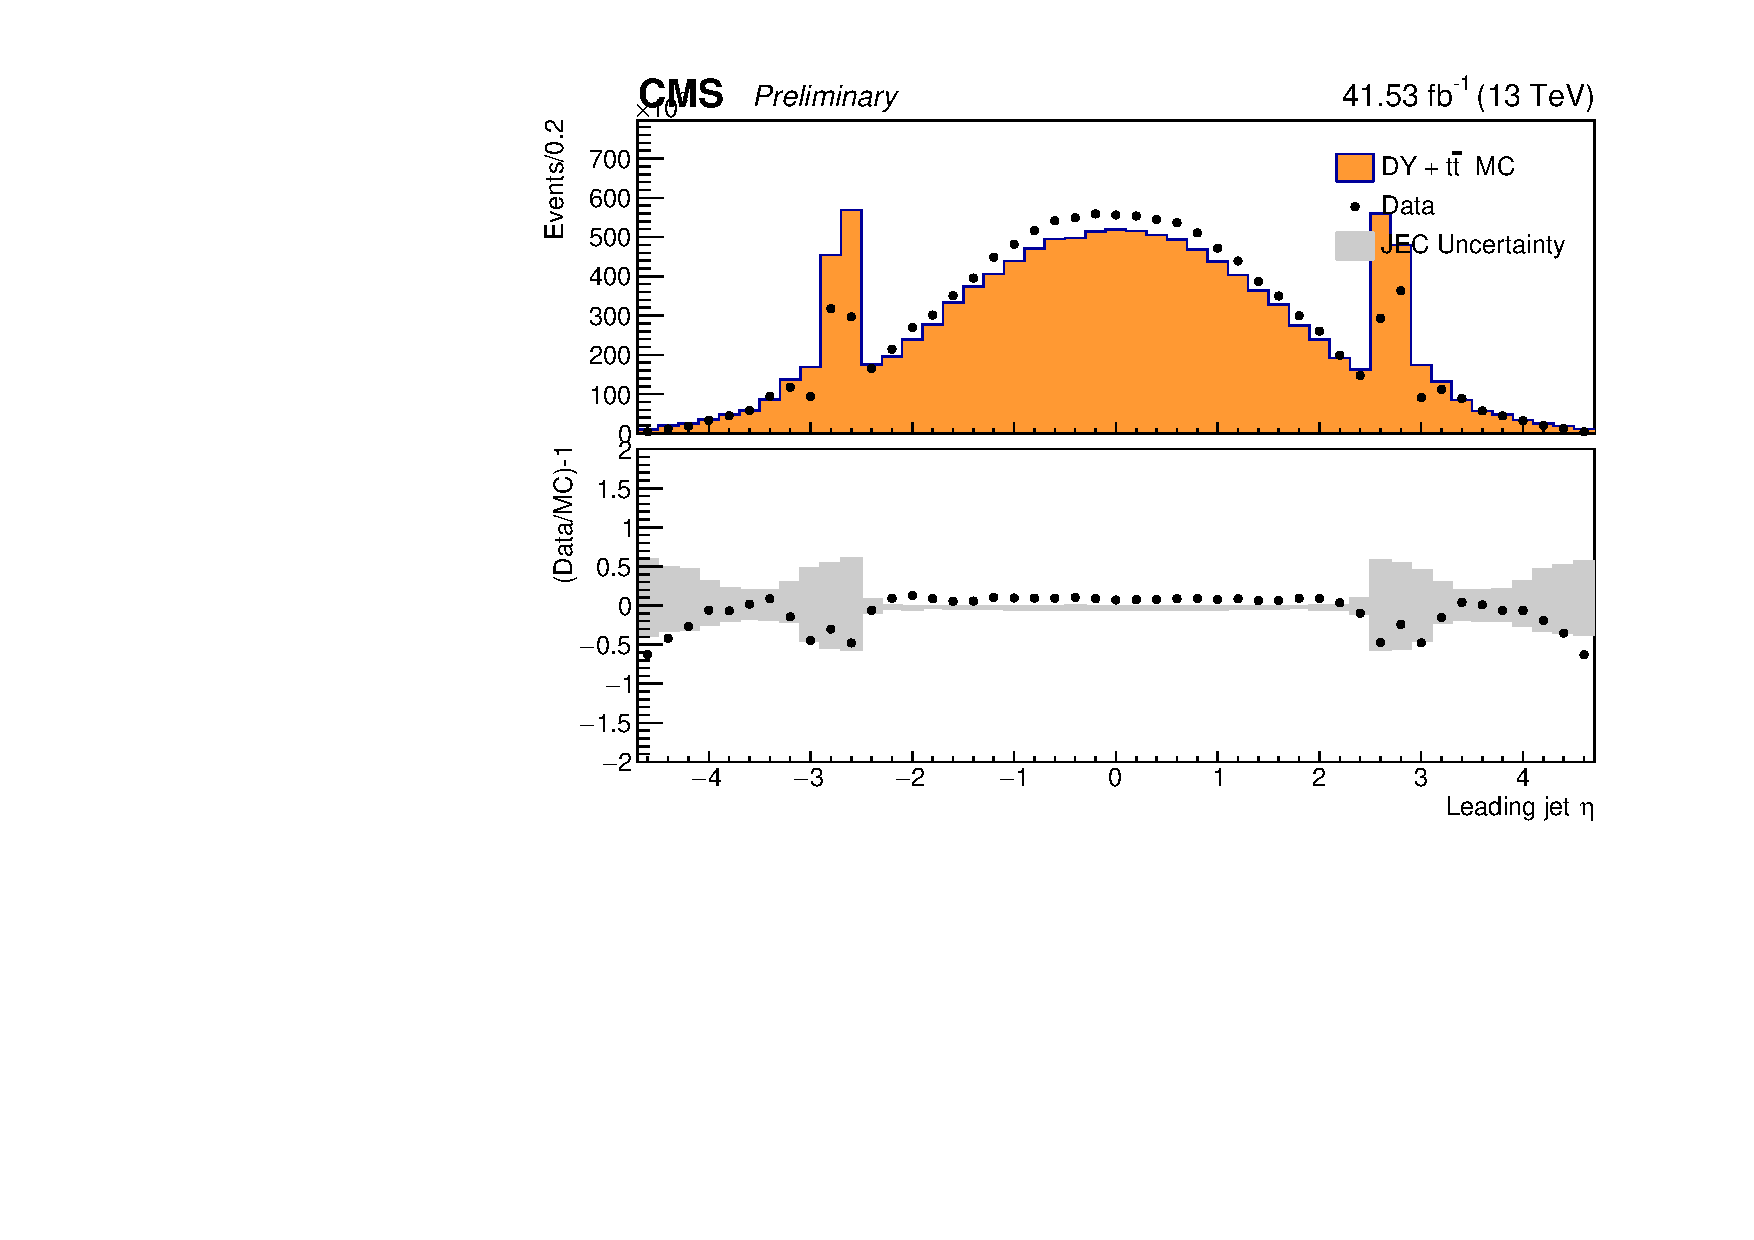
\includegraphics[width=0.49\linewidth]{Figures/Jets/2017_leadingJetEta_jetID_puID.pdf} \\
%%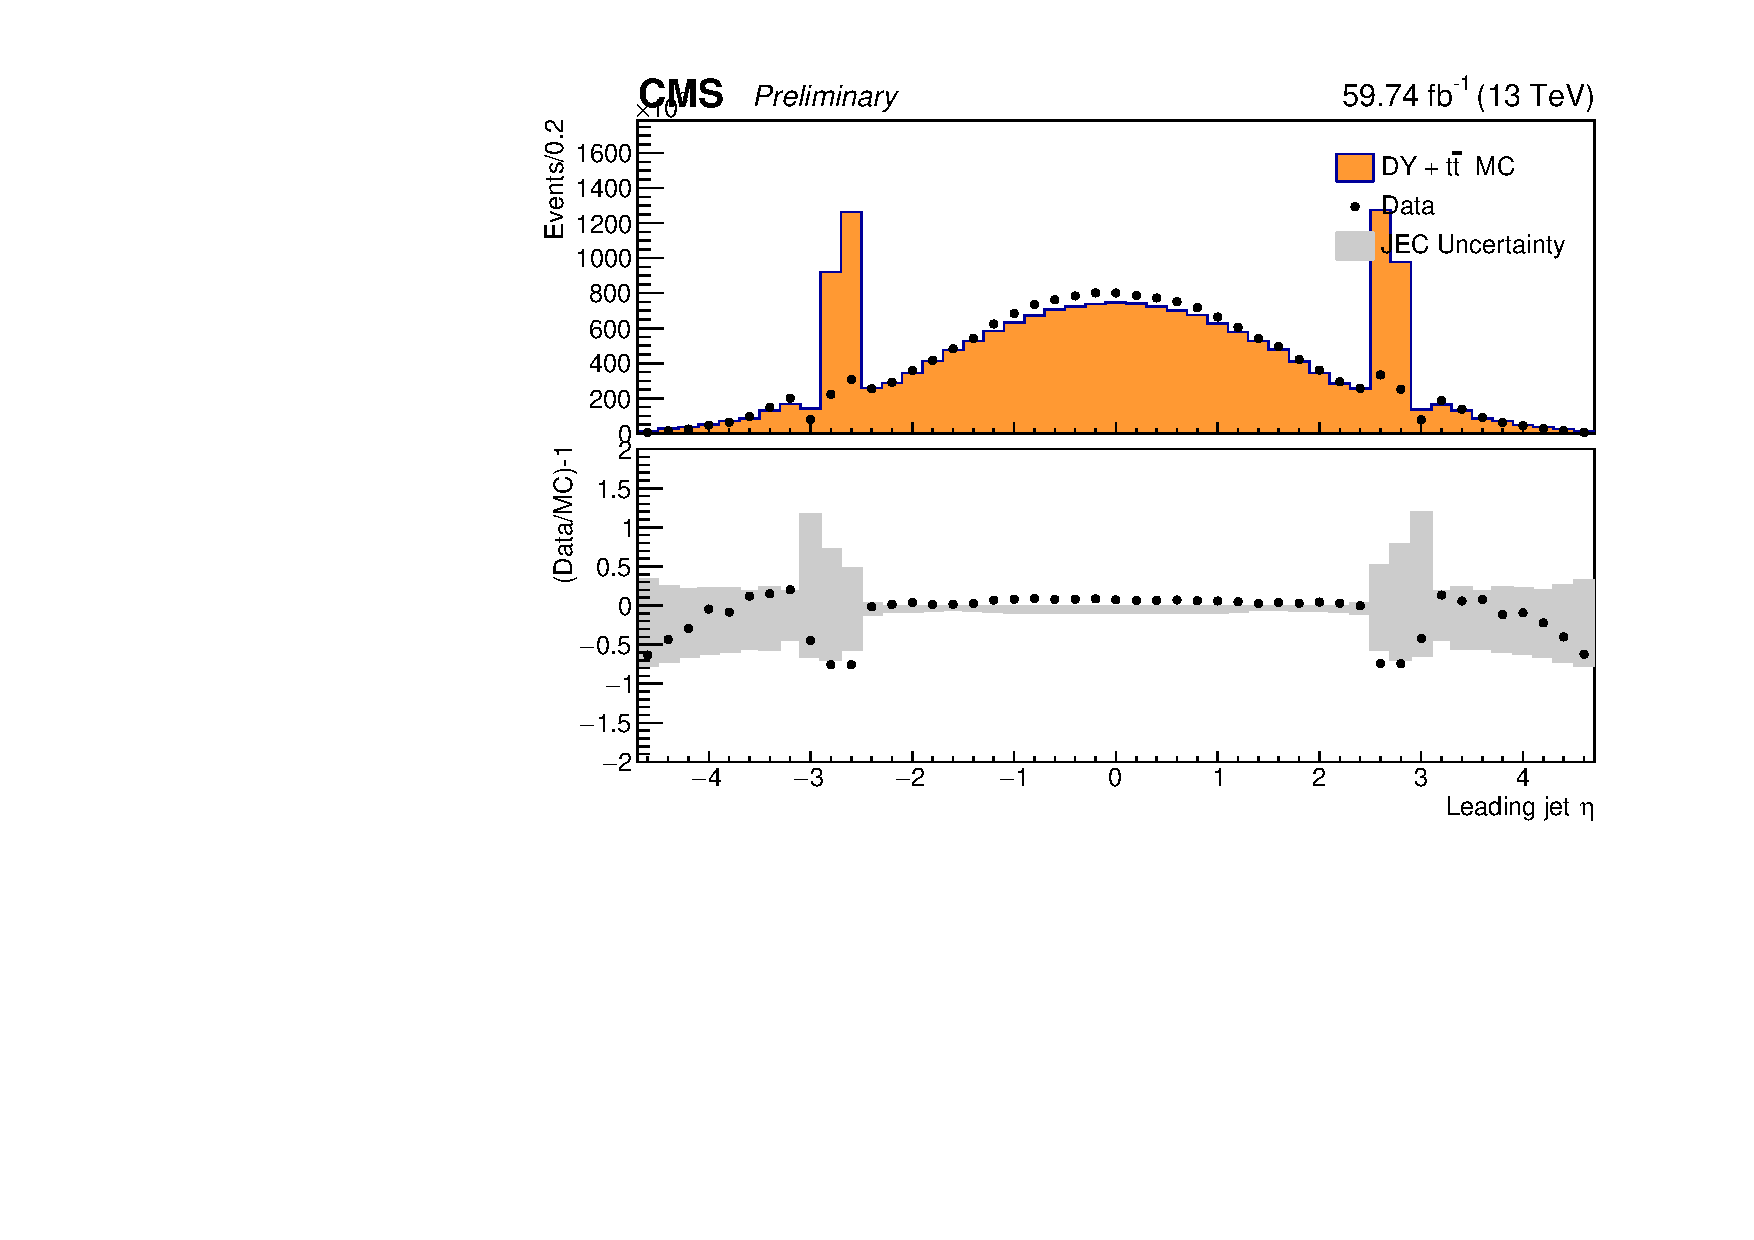
\includegraphics[width=0.49\linewidth]{Figures/Jets/2018_leadingJetEta_jetID_puID.pdf}
%%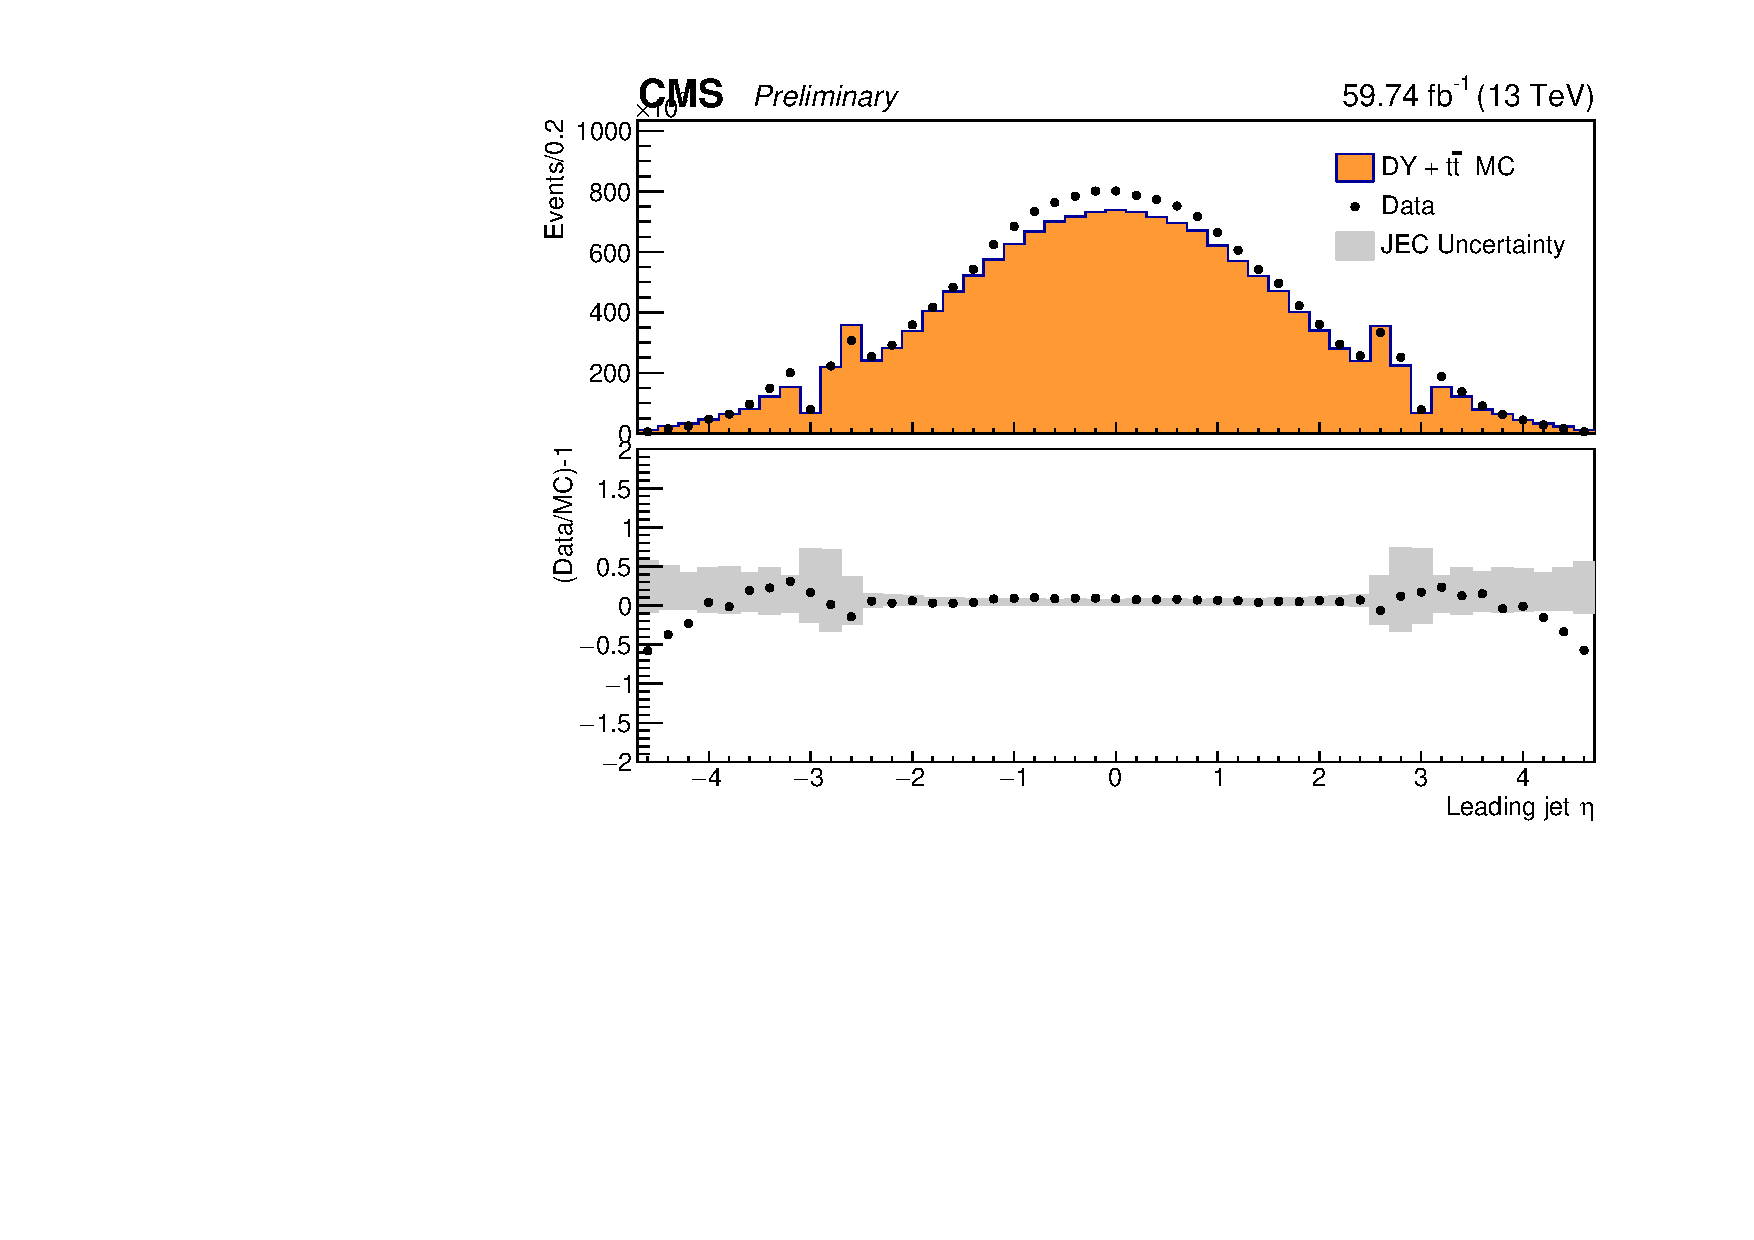
\includegraphics[width=0.49\linewidth]{Figures/Jets/2018_noJER_leadingJetEta_jetID_puID.pdf}
%%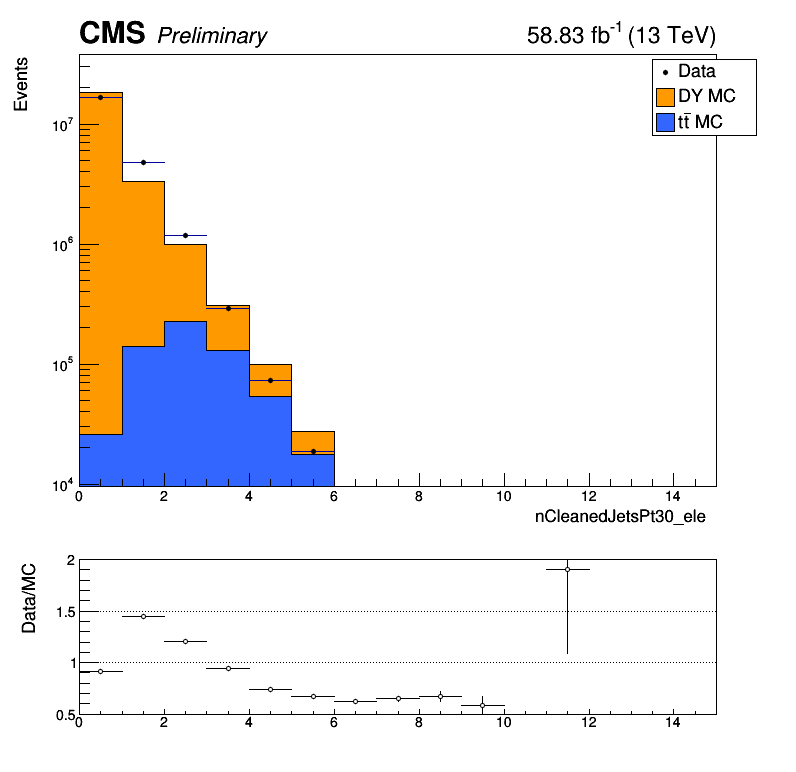
\includegraphics[width=0.49\linewidth]{Figures/Jets/nCleanedJetsPt30_ele.png} 
%%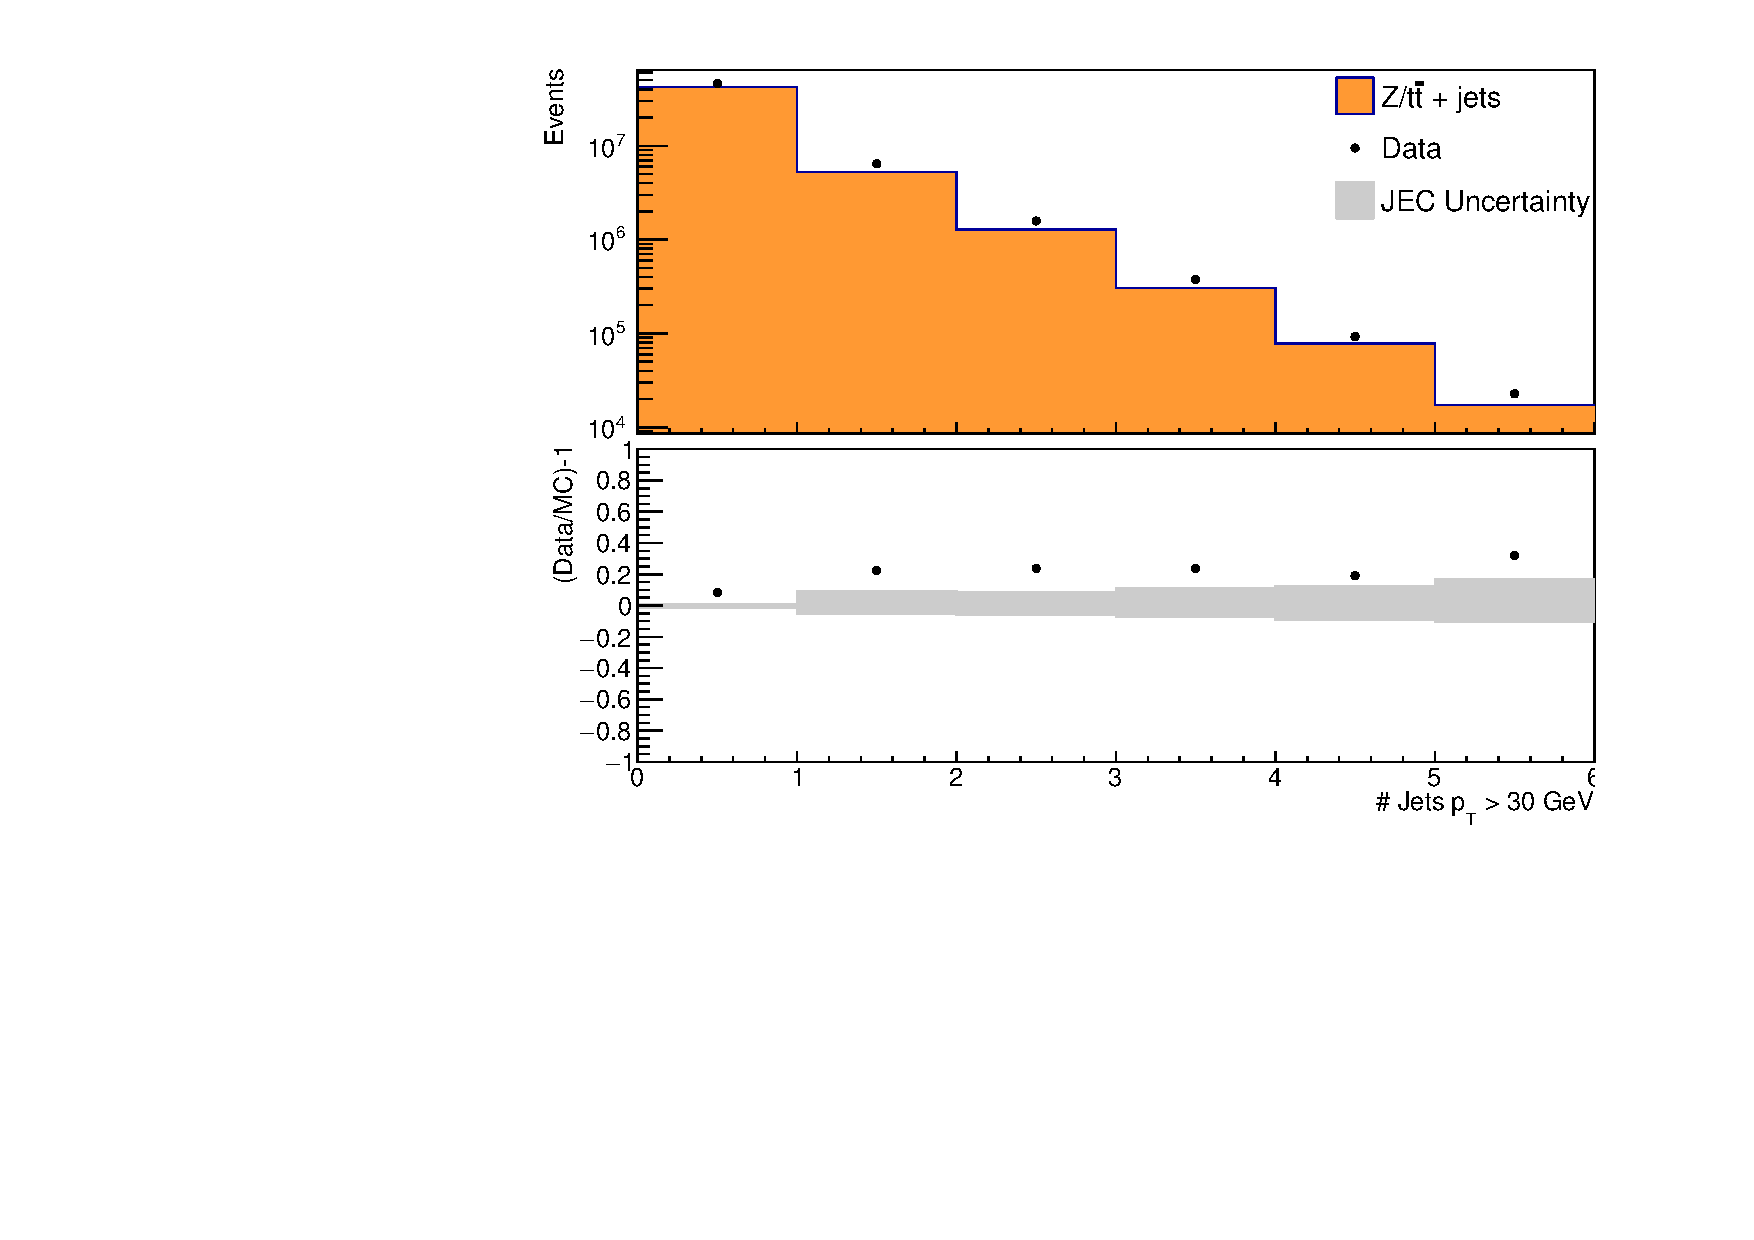
\includegraphics[width=0.69\linewidth]{Figures/Jets/nCleanedJetsPt30.pdf} \\
%%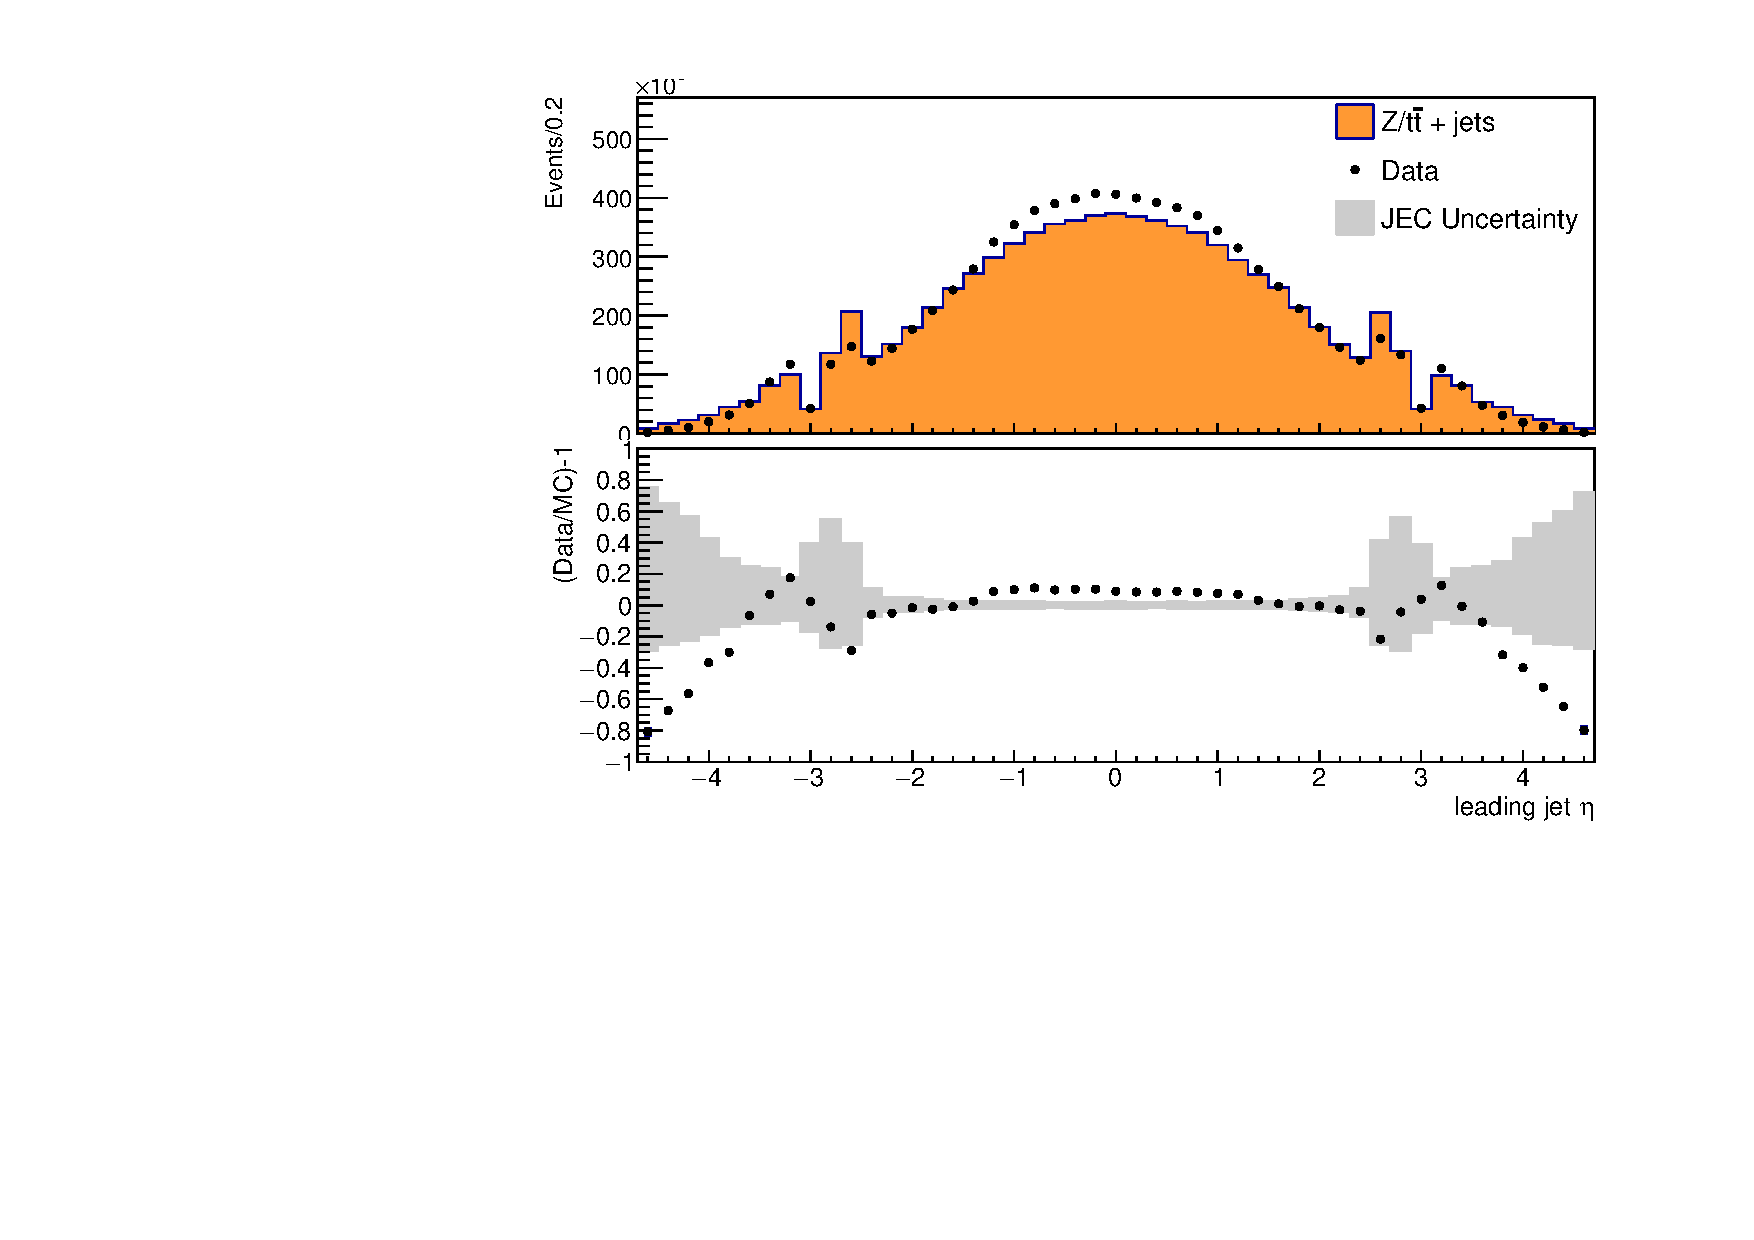
\includegraphics[width=0.69\linewidth]{Figures/Jets/leadingJet_Eta.pdf} 
%%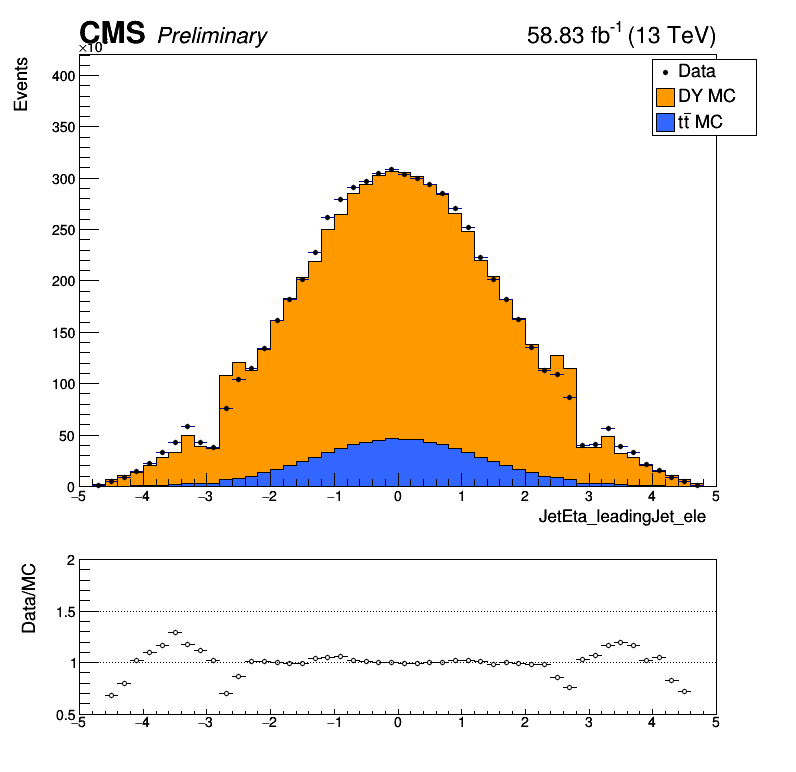
\includegraphics[width=0.49\linewidth]{Figures/Jets/JetEta_leadingJet_ele.png} \\ 
%%\includegraphics[width=0.49\linewidth]{Figures/Jets/Histo_etaj1_2mu_dataeff.pdf}
%%\caption{Comparison between data and MC for number of jets with $p_T>30$~GeV (top) and leading jet $\eta$ (bottom) in Z$\rightarrow \ell\ell$ +jets events.
%\caption{Comparison between data and MC for the leading jet $p_T$ (left) and jet $\eta$ (right) for 2016 (top), 2017 (middle) and 2018 (bottom). Z$\rightarrow \ell\ell$ +jets events are used. 
%% (left) and Z$\rightarrow\mu\mu$ + jets events (right). 
%MC is normalized to data. Jet ID and Jet PUID are applied. MC samples include DY and ttbar. Data/MC ratio plots are shown in the bottom of each plots, together with the uncertainties (shaded histograms) from Jet Energy Corrections.
%%\textbf{FIXME: Add the uncertainty band in the ratio plot.}
%\label{fig:jets}}
%\end{figure}
%
%\begin{figure}[!h]
%\centering
%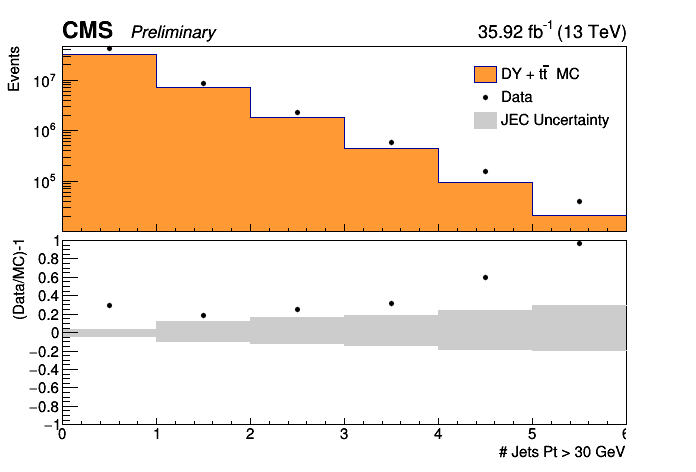
\includegraphics[width=0.49\linewidth]{Figures/Jets/nCleanedJetsPt30_2016June24.png} \\
%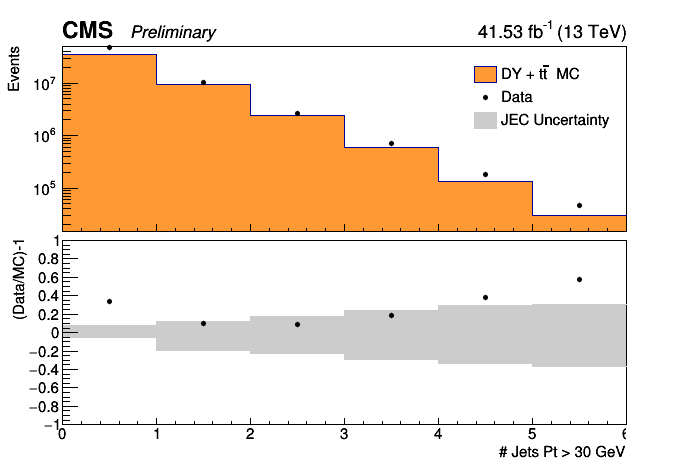
\includegraphics[width=0.49\linewidth]{Figures/Jets/nCleanedJetsPt30_2017June24.png} \\
%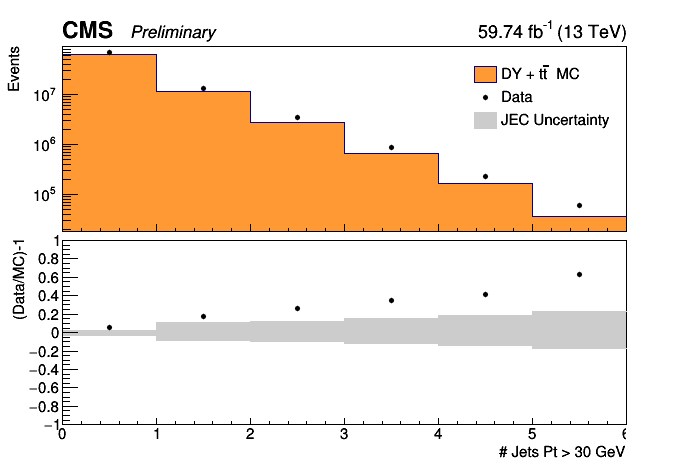
\includegraphics[width=0.49\linewidth]{Figures/Jets/nCleanedJetsPt30_2018June24.png} \\
%
%\caption{Comparison between data and MC for the jet multiplicity for 2016 (top), 2017 (middle) and 2018 (bottom). Z$\rightarrow \ell\ell$ +jets events are used. 
%% (left) and Z$\rightarrow\mu\mu$ + jets events (right). 
%MC is normalized to data. Jet ID and Jet PUID are applied. MC samples include DY and ttbar. Data/MC ratio plots are shown in the bottom of each plots, together with the uncertainties (shaded histograms) from Jet Energy Corrections.
%%\textbf{FIXME: Add the uncertainty band in the ratio plot.}
%\label{fig:jetsN}}
%\end{figure}
%
%%\begin{figure}[!h]
%%\centering
%%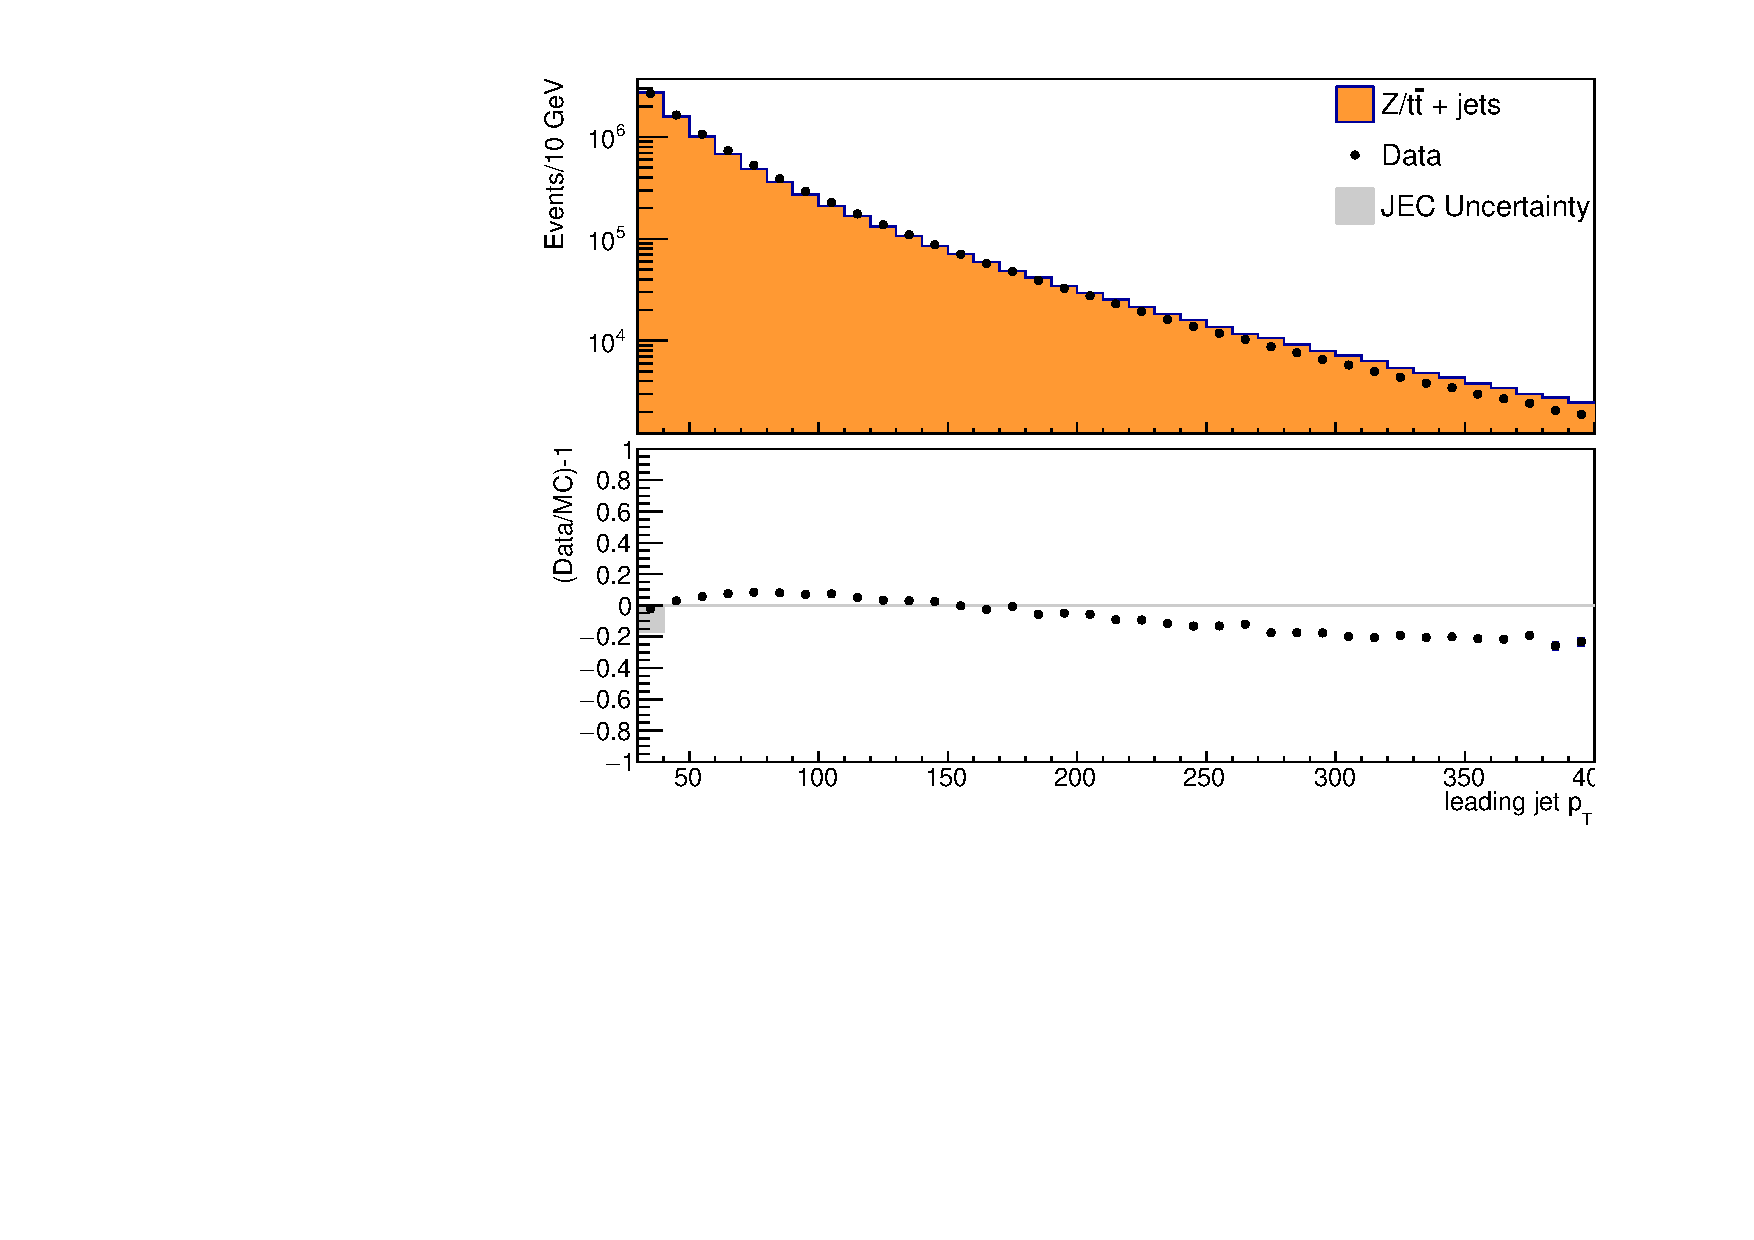
\includegraphics[width=0.69\linewidth]{Figures/Jets/leadingJet_Pt.pdf} \\
%%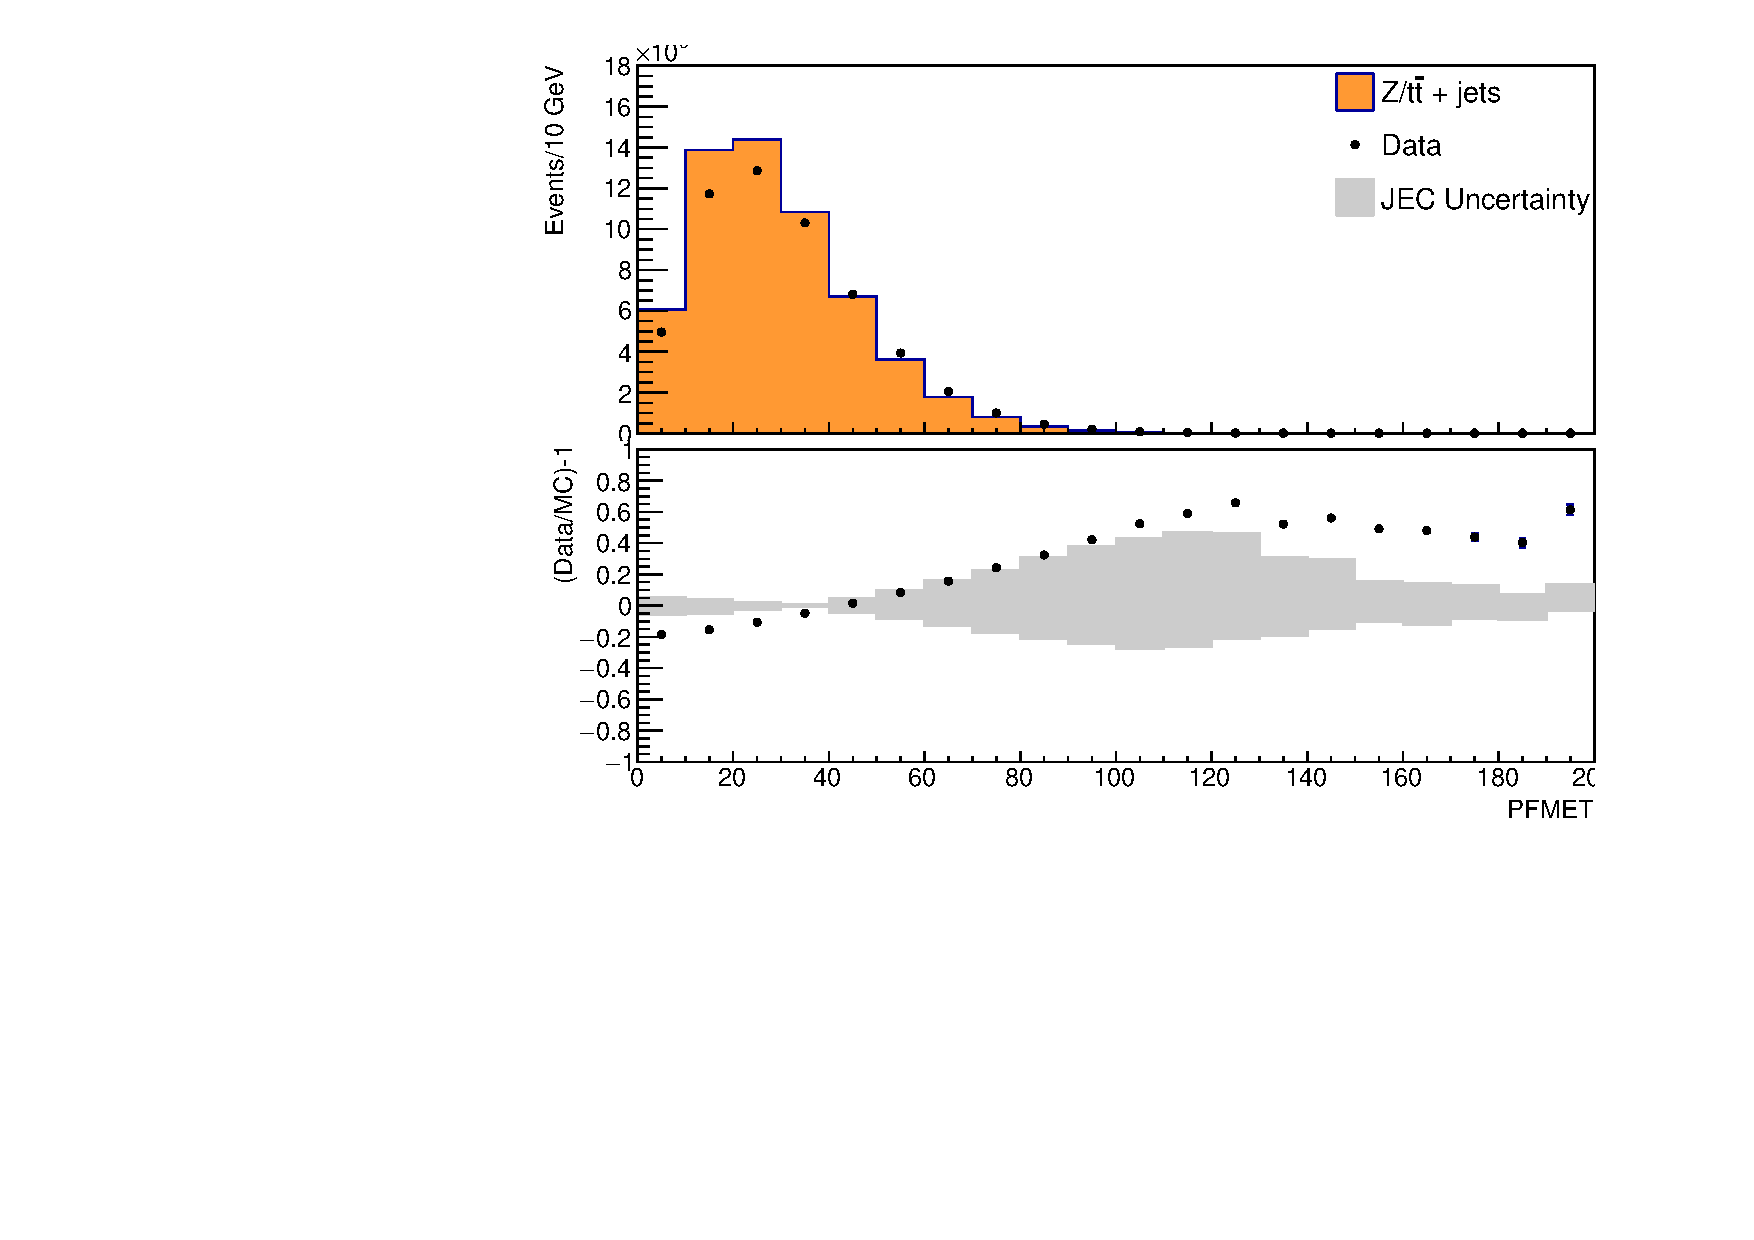
\includegraphics[width=0.69\linewidth]{Figures/Jets/PFMET.pdf} 
%%\caption{Comparison between data and MC for the leading jet $p_T$ (left) and the PFMET with 
%%Jet ID and Jet PUID applied. MC samples include DY and ttbar. MC is normalized to data. Data/MC ratio plots are shown in the bottom of each plots, together with the uncertainties (shaded histograms) from Jet Energy Corrections.
%%\textbf{FIXME: Add the uncertainty band in the ratio plot.}
%%\label{fig:met}}
%%\end{figure}
%
%%Horns around $\eta$~3 can be seen. It actually happens that Jet PUID and Jet ID were not applied in the plots above. 
%%We thus reprocessed part of the data (Run C only) and the Drell-Yan MC with the latest recommendations for the JetMET POG and we obtained the plots on the Fig~\ref{fig:jetsID}:
% 
%%\begin{figure}[!h]
%%\centering
%%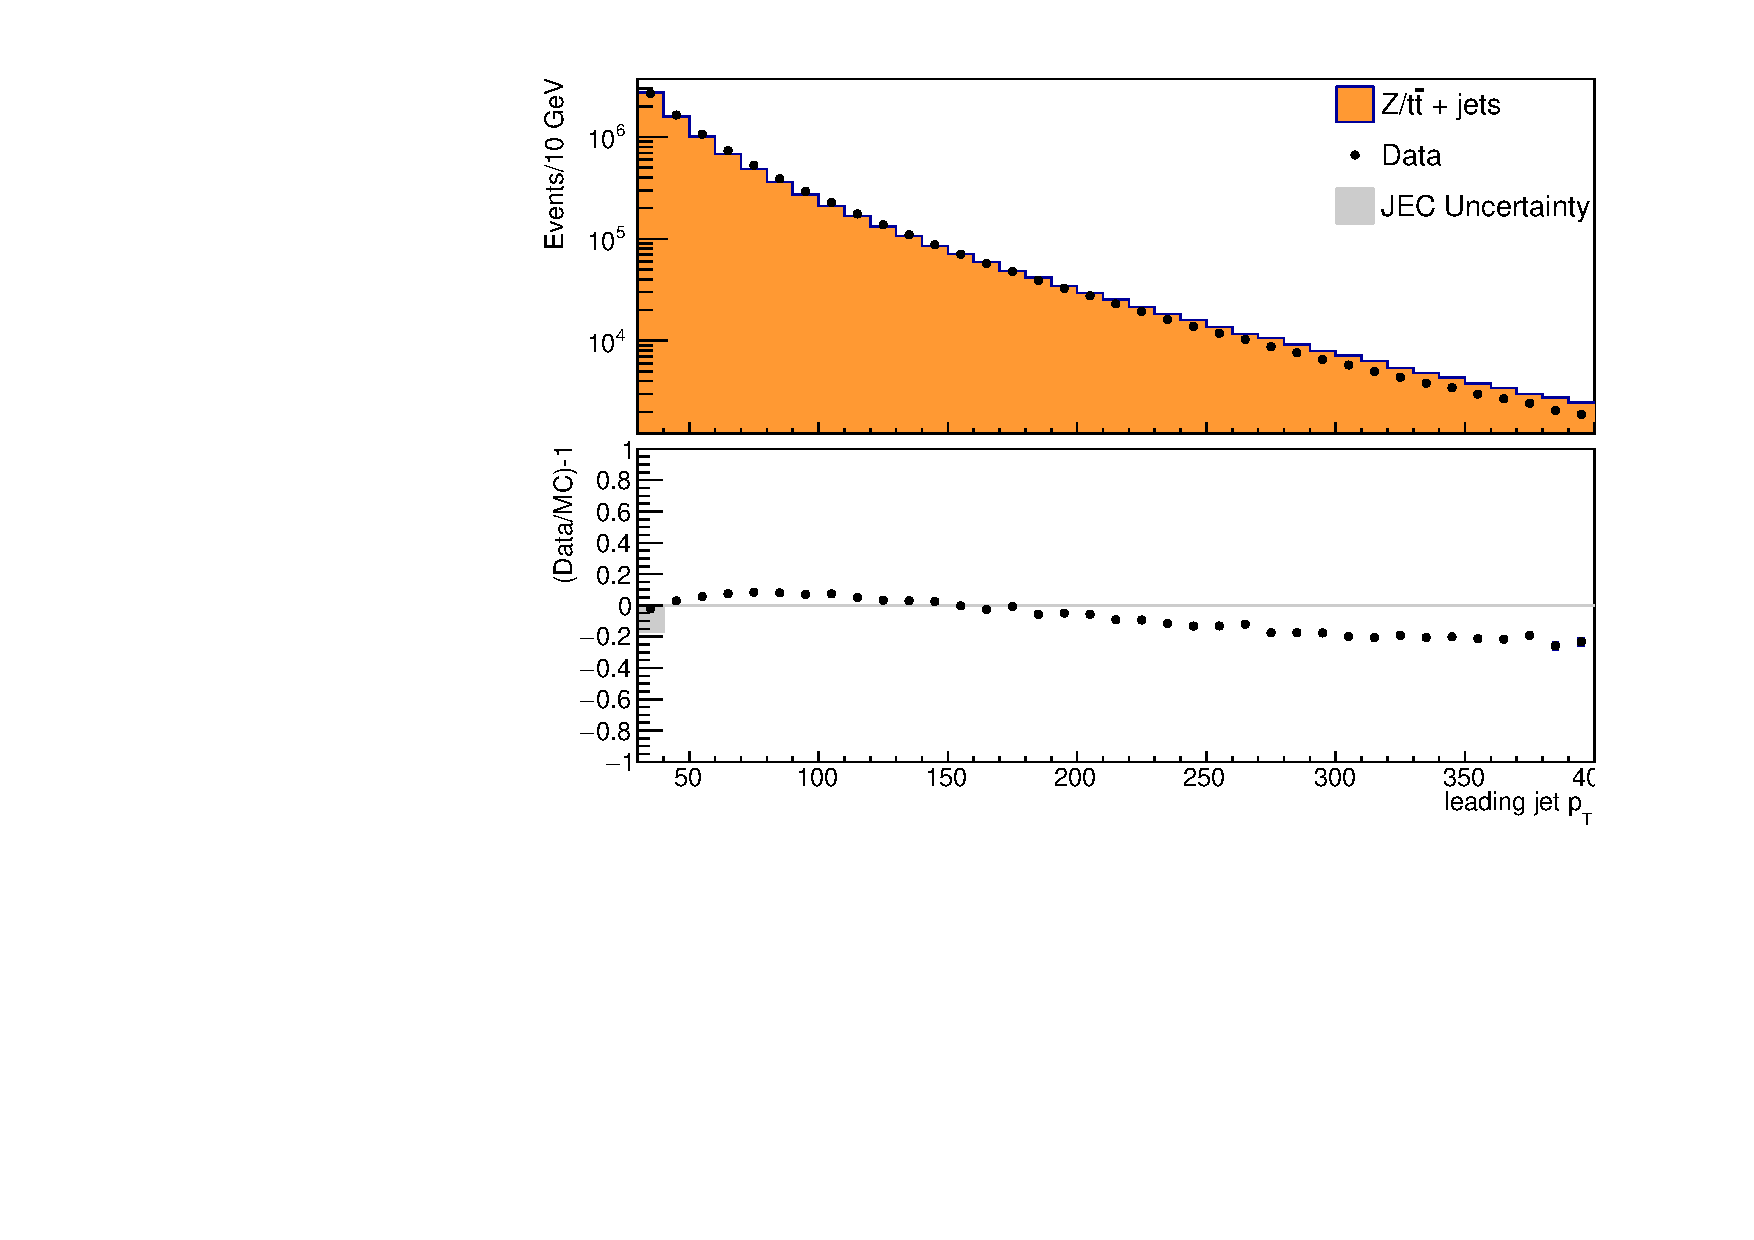
\includegraphics[width=0.4\linewidth]{Figures/Jets/leadingJet_Pt.pdf} %isto_etaj1_2e_dataeff.pdf}
%%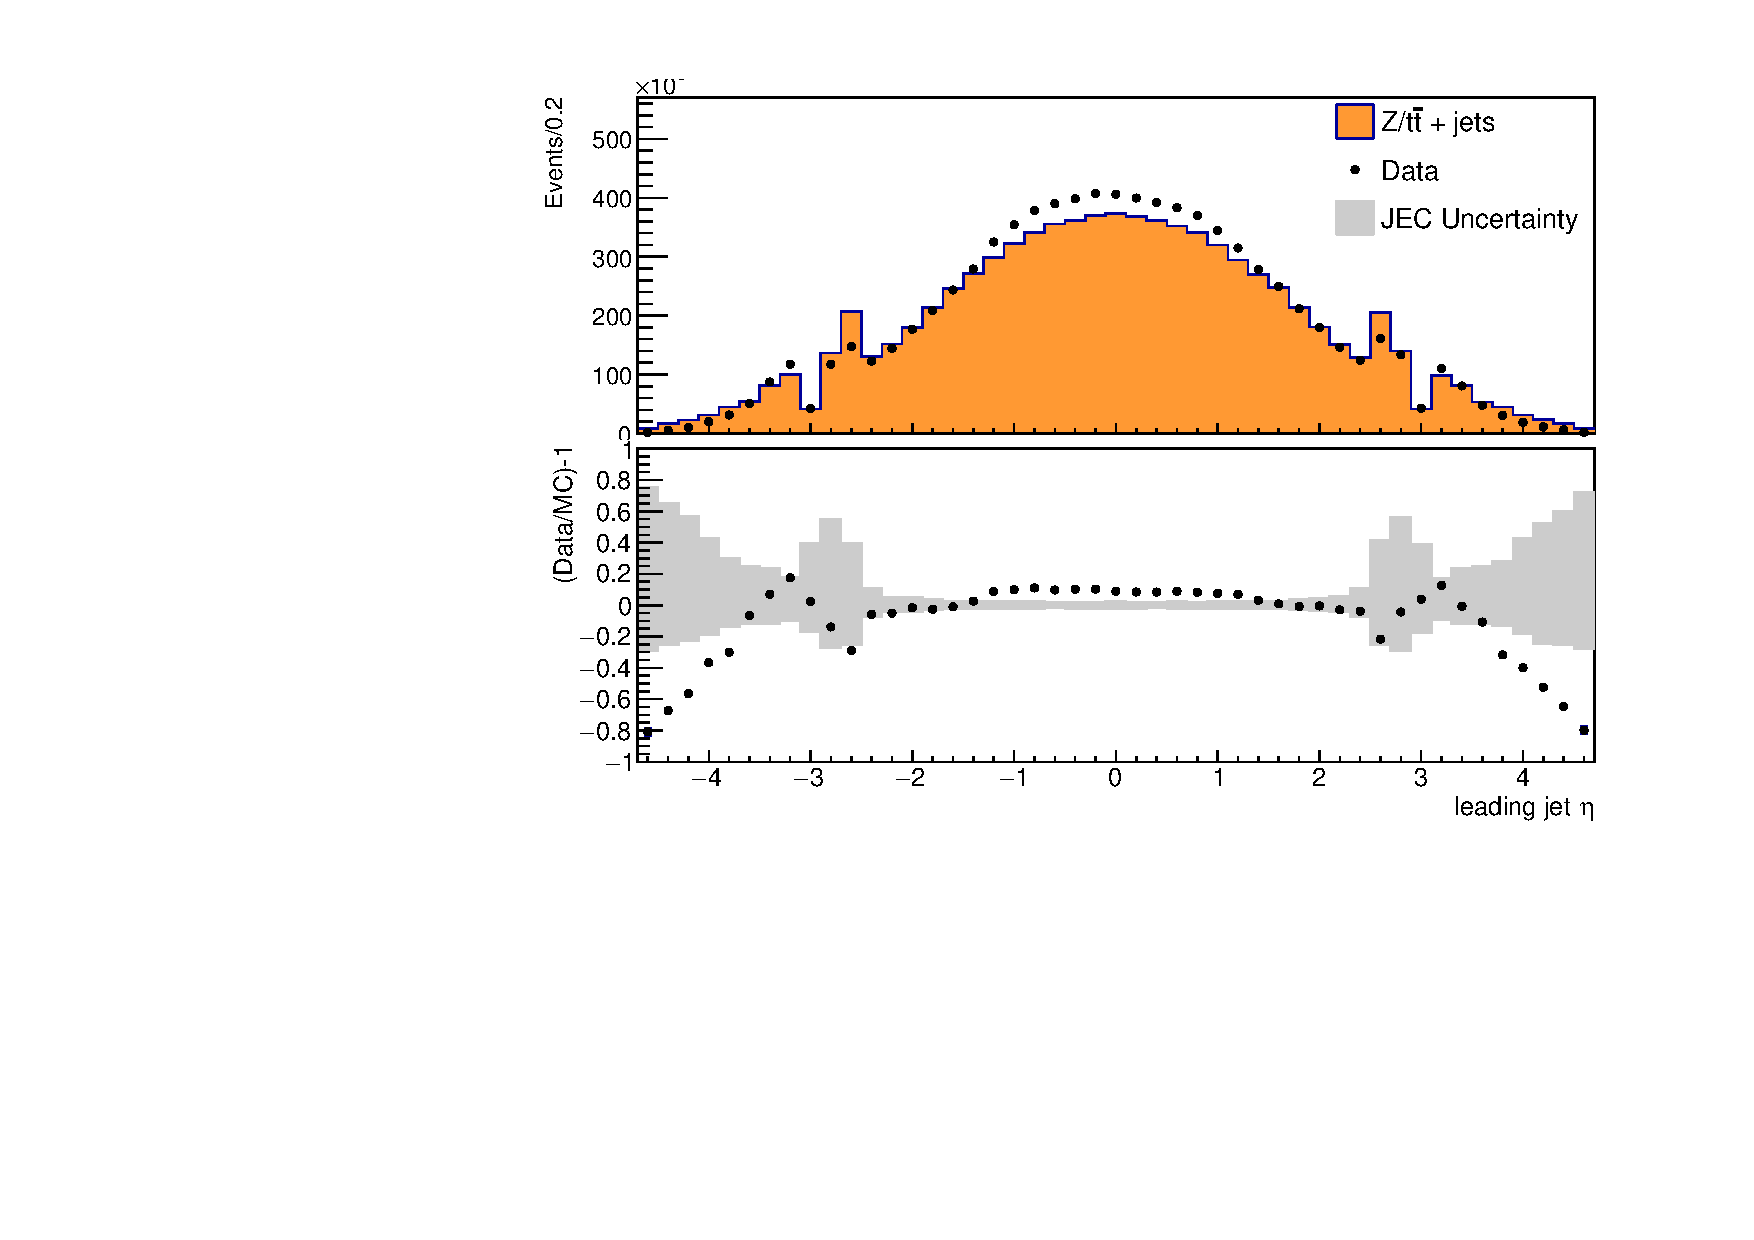
\includegraphics[width=0.4\linewidth]{Figures/Jets/leadingJet_Eta.pdf} \\
%%\includegraphics[width=0.4\linewidth]{Figures/Jets/leadingJet_Phi.pdf}
%%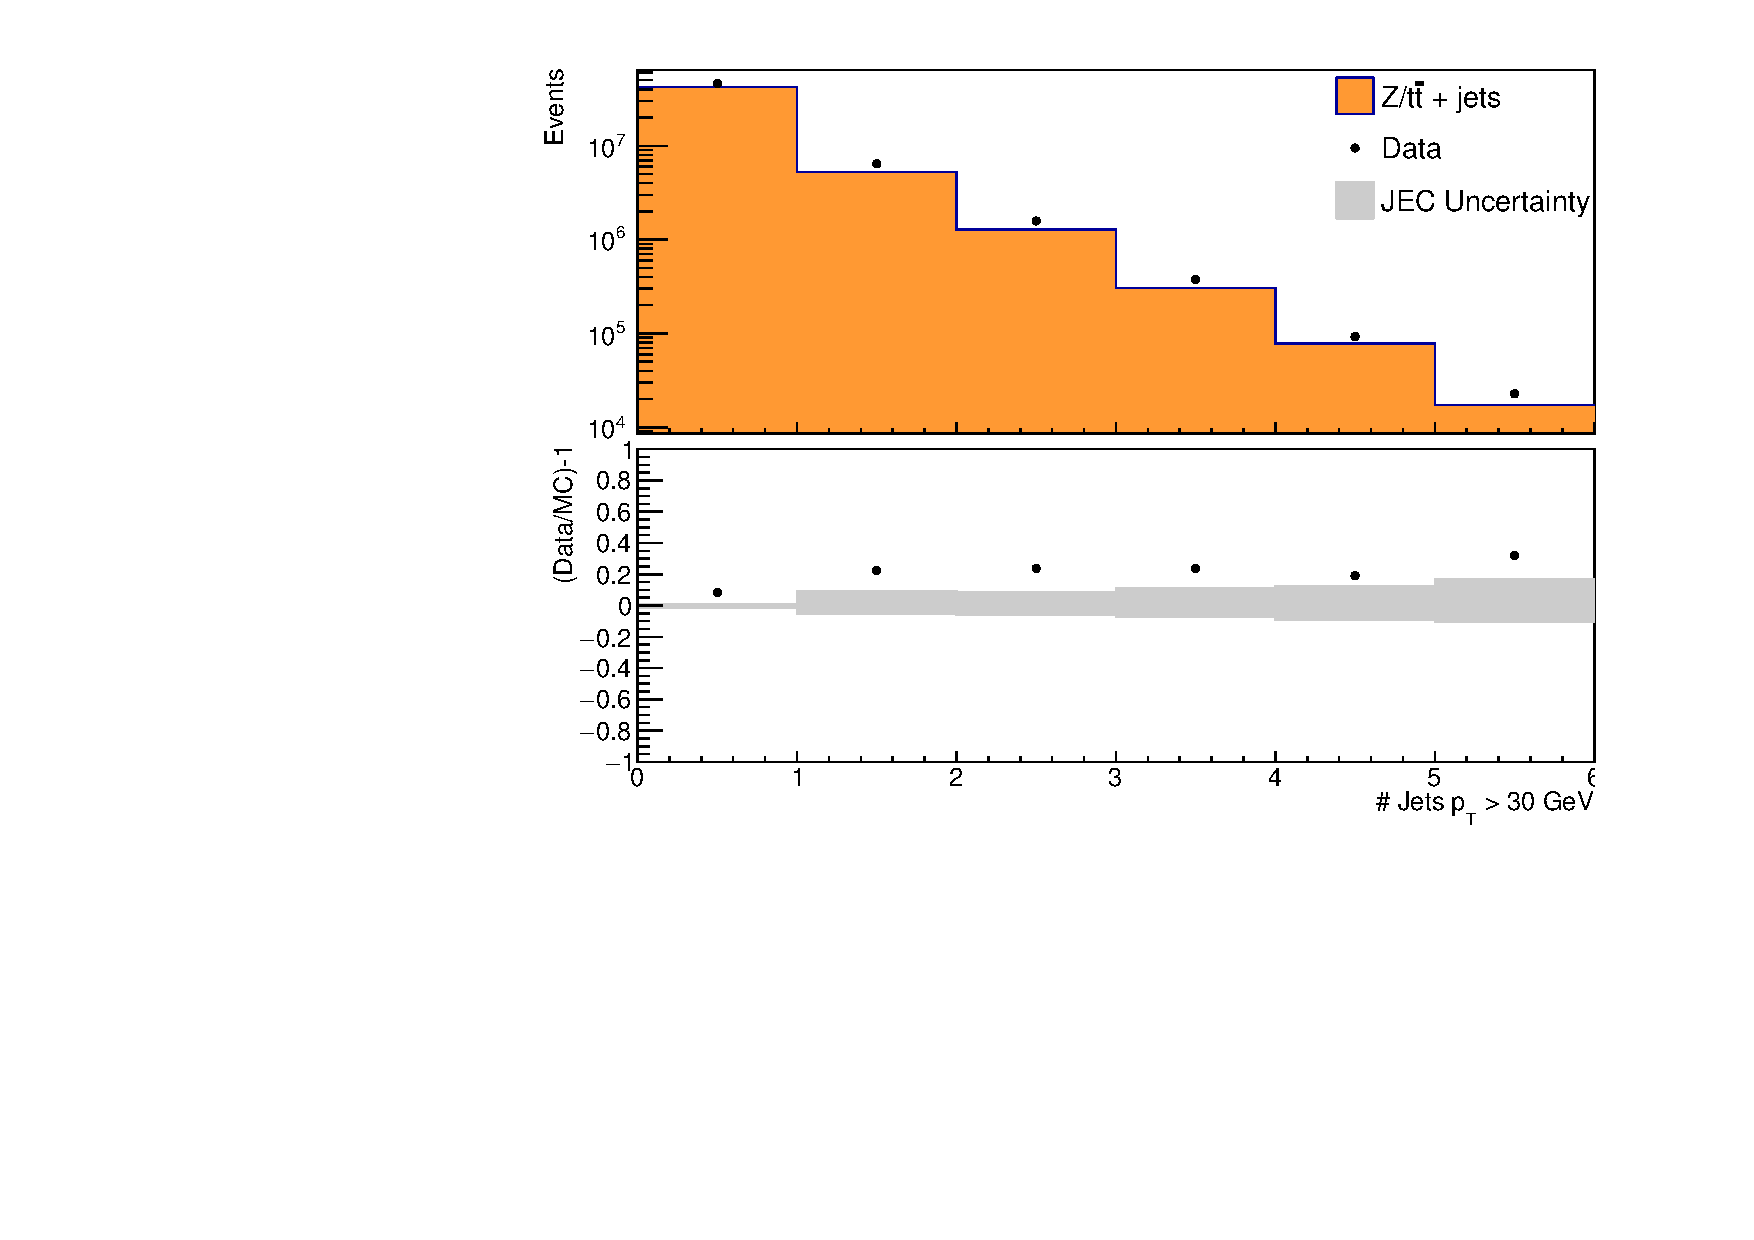
\includegraphics[width=0.4\linewidth]{Figures/Jets/nCleanedJetsPt30.pdf} \\
%%\includegraphics[width=0.4\linewidth]{Figures/Jets/leadingJet_Btag.pdf}
%%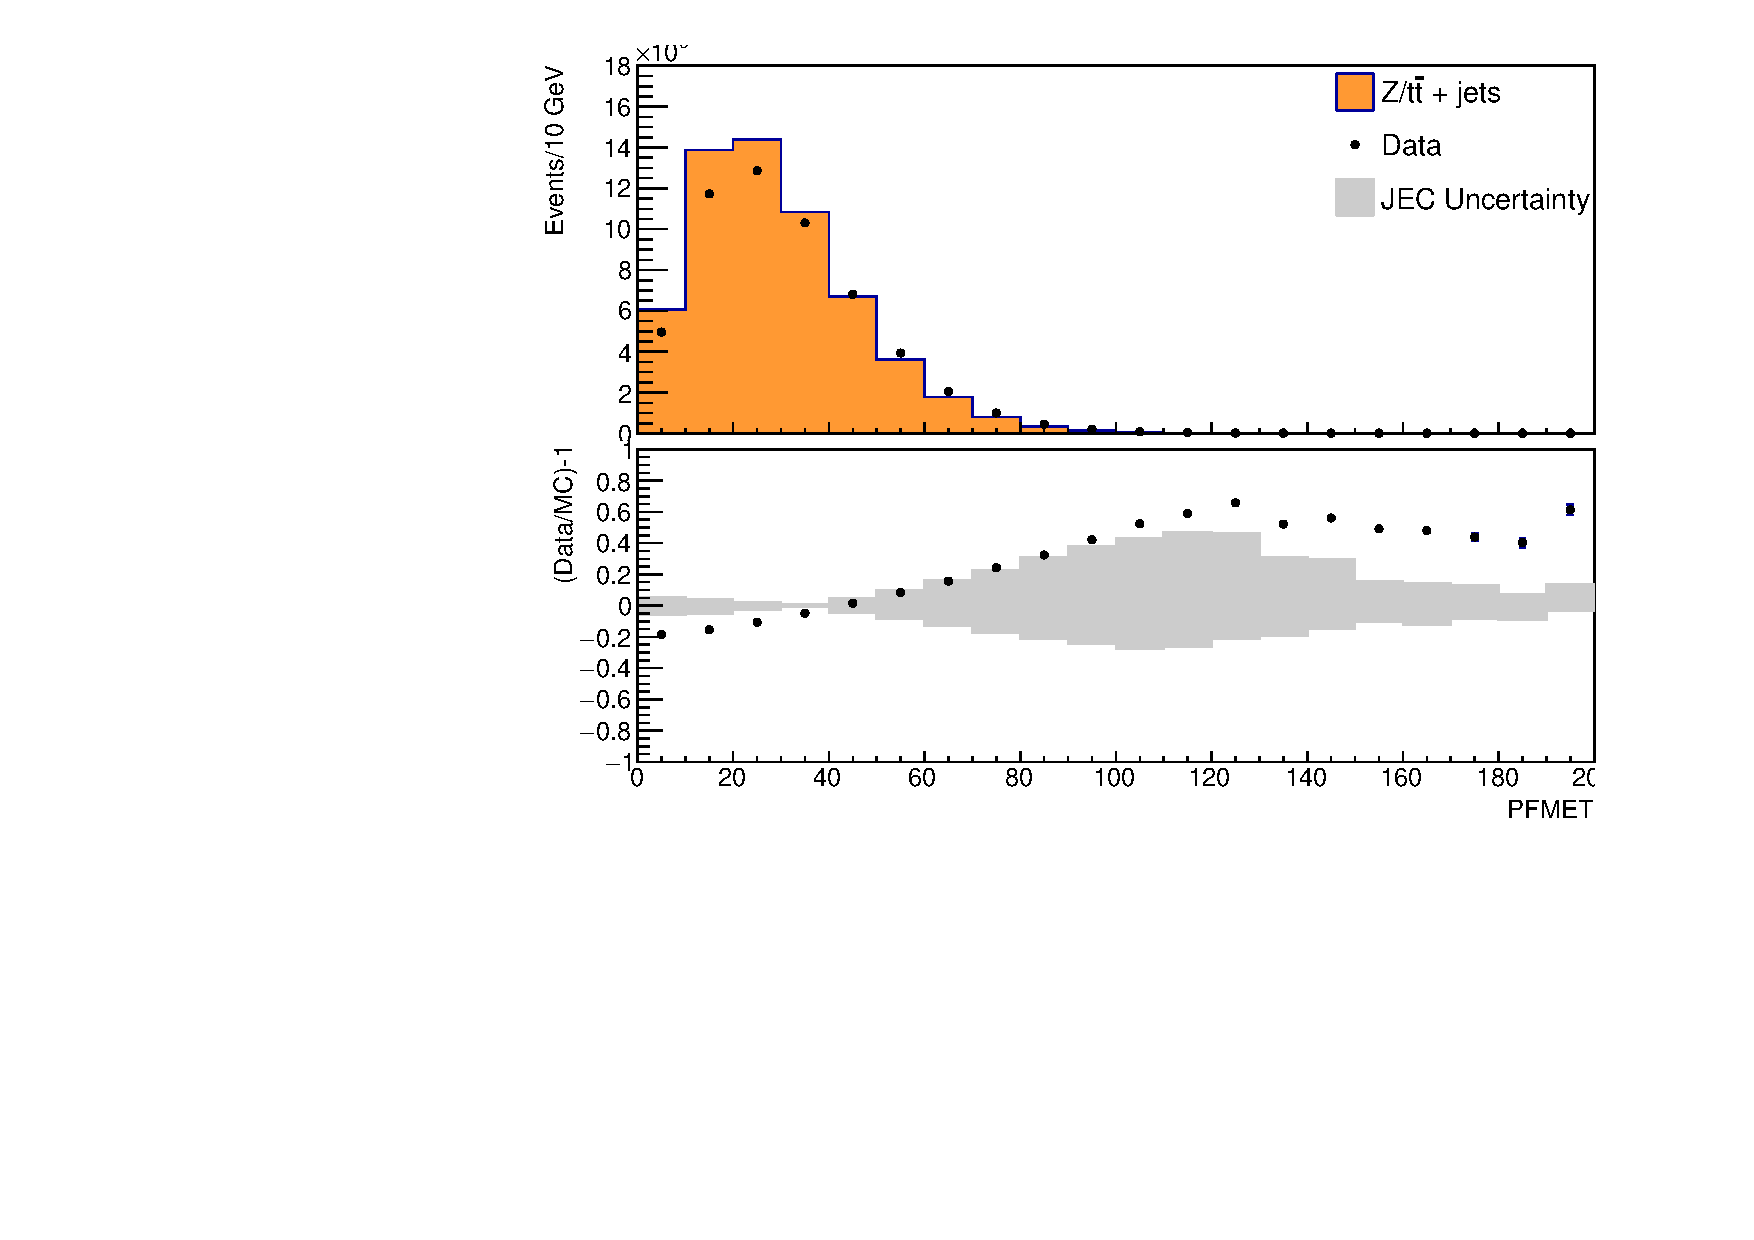
\includegraphics[width=0.4\linewidth]{Figures/Jets/PFMET.pdf}  \\
%%\includegraphics[width=0.49\linewidth]{Figures/Jets/Histo_etaj1_2mu_dataeff.pdf}
%%\caption{Comparison between data (RunC only) and MC for leading jet $p_T$ (top left), leading jet $\eta$ (top right), leading jet $\phi$ (middle left), number of jets with $p_T>30$~GeV (middle right), output of the b-tagger of the leading jet (bottom left) and PFMET (bottom right) in Z + jets events. Jet ID and Jet PUID are applied. $\ensuremath{\cPqt\bar{\cPqt}}$ MC sample is not included. 
%%\label{fig:jetsID}}
%%\end{figure}
%
%%The agreement is now much better and only remain some mismatch in the tais, as one could expect for the missing contribution from $\ensuremath{\cPqt\bar{\cPqt}}$. While the results presented after do not include the JetPUID and JetID, we will include them in the next iteration, together with the final Scale Factors and object correction provided by the various POGs. 
